% Original template ripped from:
% http://www.cs.technion.ac.il/~yogi/Courses/CS-Scientific-Writing/examples/simple/simple.htm


\date{\today}

\documentclass[12pt]{report}

\usepackage{caption}
\usepackage{graphicx}
\usepackage{lmodern}
\usepackage{listings}
\usepackage{idrislang}
\usepackage{amsfonts,amsthm,amsmath}
\usepackage[margin=3cm]{geometry}
\usepackage[en,nat,farve,titelside]{ku-forside}
\usepackage[mark,missing={CONFIGURE gitinfo2 PACKAGE}]{gitinfo2}
\usepackage[nounderscore]{syntax}
\usepackage{mdframed}
\usepackage{float}
\usepackage[toc,page]{appendix}

\renewcommand{\gitMark}{\gitBranch\ :\ \gitHash\ \textbullet{}\ (\gitAuthorDate)\ \textbullet{}\ \gitFirstTagDescribe}

\newtheorem{defn}{Definition}[chapter]
\newtheorem{thm}[defn]{Theorem}
\newtheorem{cor}[defn]{Corollary}
\newtheorem{lem}[defn]{Lemma}

\opgave{M.Sc. Thesis}
\forfatter{
        Casper Holmgreen and Knut Liest\o l
        % going by alphabetical order here....
}
\title{DPDT: Differential Privacy with Dependent Types}
\undertitel{or: How I Learned to Stop Worrying and Love Dependent Types}
\vejleder{Supervised by Ken Friis Larsen}
\dato{November 11, 2015}


\begin{document}
\maketitle

\lstset{language=idris,
basicstyle=\ttfamily\footnotesize,
frame=single,
numbers=left,
breaklines=true,
postbreak=\raisebox{0ex}[0ex][0ex]{\ensuremath{\color{red}\hookrightarrow\space}}
}

\graphicspath{{assets/}}

\begin{abstract}
With more personal data being stored in the ``cloud'' every day, privacy is becoming an important topic for public discussion.
Private data is potentially quite useful, but cannot be released in its raw form due to privacy concerns.
Differential privacy is an emerging field of research aiming to protect the privacy of individuals participating in a database while maximizing its utility.

PINQ is a framework for the C\# enforcing differential privacy constraints over top of the popular integrated query language, LINQ.
Users are able to build complex, differentially-private queries from a few carefully implemented primitives.
PINQ data providers are then able to dynamically reject queries which could put private information at risk.

Type systems can statically verify programs for varying degrees of correctness.
Dependent types are a particularly powerful feature of certain type systems which allows types to be predicated on values.
Because of this, we believe dependent types are a natural fit for capturing differential privacy metrics.

We present a prototype of a differentially-private query language, DPDT, in the dependently-typed, functional programming language Idris.
DPDT is loosely modelled on PINQ.
However, whereas PINQ verifies privacy constraints dynamically, DPDT is able to do it statically.
In addition, DPDT is completely type-safe in all of its relational algebra operations.

We outline the benefits and drawbacks to using dependent types for enforcing differential privacy.
Limitations of DPDT in comparison to PINQ are backend support, and expressibility of dynamically terminating algorithms.
However, a large number of side-channel attacks that PINQ is unable to stop are impossible in DPDT.
\end{abstract}

\clearpage
\tableofcontents
\clearpage
\listoffigures
\clearpage

\chapter{Introduction}\label{sec:introduction}

With each passing day, more and more of our personal information is being collected, cataloged and analyzed by an ever increasing number of interested parties.
Their interests range from selective marketing to collecting business performance metrics, and from publicly-funded academic research to unauthorized and potentially illegal surveillance.
We aren't able to curate or control the data they are collecting about us.
In fact, the ubiquity of automatic data collection probably gives them a better picture of you than they would get if you did curate and volunteer the data.
Therefore, as the producers and descriptees of this data, we should be concerned with how it is being used.

There are many creative ways to use data and not all of them align so simply with ``good'' and ``bad''.
Additionally, there is some information that a few trusted people (or systems) must know, but we might not necessarily want our nosy neighbor knowing.
Publicly available data can also help researchers to discover or verify solutions for various societal problems.

Consider Alice's medical records.
Alice's doctor should have access to this very sensitive information, but her neighbor and insurance salesman probably should not.
Recognizing the importance of the right to privacy, some countries have imposed legal privacy requirements on systems maintaining sensitive information, such as medical records (e.g. the Health Insurance Portability and Accountability Act (HIPAA) in USA).
However, Alice's medical records contain valuable data for researchers aiming to understand health trends in our society, but they can't access it without violating her privacy.

Public health researchers would be able to monitor and analyze the long-term health trends of a population over time.
Epidemiologists could detect infectious diseases early and prevent their spread.
The benefits of increased data availability are not limited to public health, either.
Databases containing large amounts of sensitive information can be tremendously valuable for researchers looking into a variety of important questions.

Big data offers us an amazing opportunity for learning about us, but how do we do it without also learning about Alice (as an individual)?
Differential privacy is an active field of research, with input from many different disciplines, that aims to answer this question\cite{journals/cacm/Dwork11}.
The goal of differential privacy is to minimize the risk for the individual while maximizing the utility of the data.

% TODO 1 : add problem statement
% TODO 1 : maybe move contributions up here? or at least outline rest of chap.
This thesis ...

\section{Differential Privacy}\label{sec:intro-diffpriv}

The question of how to provide access to sensitive data is not a new one.
Many techniques for data sharing with privacy constraints have been explored.
They can generally be partitioned into two main approaches: \textit{interactive} (i.e. requires the participation of a ``middle man'') and \textit{non-interactive} (i.e. can be released directly to the public).

One example of a non-interactive approach which has received significant news\footnotemark[\ref{fn:aol}] coverage\footnotemark[\ref{fn:twitter}] a few times\footnotemark[\ref{fn:netflix}] by now\footnotemark[\ref{fn:gic}], is to anonymize or otherwise ``fuzz'' a dataset before releasing it to the public.
However, it is very difficult to release a database that is both useful and private.
Other approaches suffer similar problems relating to privacy or are infeasible to maintain\cite{journals/cacm/Dwork11}.

Differential privacy differentiates itself from other private data release mechanisms by defining privacy differently.
Early approaches often modeled their definition of privacy on the concept of \textit{perfect secrecy} from cryptography: could an adversary with access to the system learn \textit{anything} about an individual?
While this definition is appealing for simplicity, it is too rigid: we actually do want somebody somewhere to learn something.
\footnote{One interesting implication of this is that the adversaries are also the analysts; i.e, we must protect against legitimate users of the system.}
Instead, differential privacy promises that Alice's participation in the database can increase her privacy risk by \textit{at most} some negligible amount.

\subsection{Indistinguishability}\label{subsec:intro-indistinguishability}

One of the centrals ideas driving differential privacy is that of indistinguishability, i.e. a query evaluated against a dataset should return more-or-less the same result regardless of whether Alice's records were included in the data.
If the result of the query with Alice included is indistinguishable from the result of the query without her, then the contents of Alice's records must be indistinguishable, too.

Indistinguishability is typically achieved by combining the true (distinguishable) result of a query with enough random noise to mask Alice's participation in the database.
However, additive noise is insufficient by itself to guarantee privacy.
An adversarial analyst could simply repeat semantically equivalent queries and average the results.
As the number of evaluated queries approaches infinity, the average will approach the true mean and Alice's personal information is now public.
This susceptibility to averaging repeated queries is one of the major factors preventing non-interactive database anonymization without greatly affecting its utility.

One interactive (and naive) solution is to maintain a query log recording every query ever evaluated against the database.
Incoming queries can then be checked against previous ones to ensure that they can be answered without violating privacy guarantees.
However, two syntactically different queries may be semantically equivalent.
There is no way for a machine to know without running the query and human labor is costly and error-prone.
Additionally, the act of refusing a query could itself be disclosive.

Another (interactive) solution is to limit the number of queries which can be run against the dataset.
However, some queries reveal more information than others, so this seems too crude.
Instead of counting the number of queries, we associate each query with a \textit{privacy cost}.
Then, each dataset is given a \textit{privacy budget}, which limits the total cost of queries that can be run against it.
Each query evaluated reduces the privacy budget by its cost until it is eventually depleted, at which point the data should be destroyed.
This is the fundamental idea behind differential privacy.

\subsection{Privacy}\label{subsec:intro-almostperfectpriv}

Early privacy research focused on preventing an adversary from learning \textit{anything} about a particular individual (e.g. Alice).
However, this goal is both impractical and impossible.
Data are valued for the potential insights we might learn;
we want analysts to learn something from the data!
We just don't want them to learn anything about a particular individual in the data.

However, this privacy objective is difficult to maintain in the presence of auxiliary information.
Ganta et al. showed that \textit{k-anonymity} and other proposed partition-based anonymization approaches are vulnerable to composition attacks\cite{ganta2008composition}.
A composition attack is performed on an ``anonymized'' data set by matching it with auxiliary data, such as data from the web, public records, or domain knowledge.
With this technique, an attacker might be able to deduce information about Alice's records in an ``anonymized'' set.

Compositions attacks are not only interesting to academics, either.
AOL\footnote{\label{fn:aol} http://arstechnica.com/business/2006/09/7835/}, Twitter\footnote{\label{fn:twitter}http://arstechnica.com/tech-policy/2009/03/pulling-back-the-curtain-on-anonymous-twitterers/}, Netflix\footnote{\label{fn:netflix}http://arstechnica.com/tech-policy/2009/09/your-secrets-live-online-in-databases-of-ruin/}, and the Massachusetts Group Insurance Commission (GIC) database\footnote{\label{fn:gic}http://web.mit.edu/sem083/www/assignments/reidentification.html} have all suffered publicly in the wakes of composition attacks.

Rather than trying to prove that an adversary cannot learn anything about an individual, differential privacy guarantees that the inclusion of an individual's records in a dataset will barely affect the adversary's ability to learn something about them.
Analysts can run differentially private algorithms against sensitive datasets knowing that no individuals' privacy will be compromised.
This is true regardless of how much auxiliary information a would-be attacker knows or \textit{might learn in the future}\cite{journals/cacm/Dwork11}.
These properties encourage honest participation during data collection.

\subsection{Example: Randomized Response}

A classic example of differentially private thinking is randomized response.
Randomized response is a technique originally proposed for encouraging survey respondents to answer potentially embarassing or legally complicated questions honestly\cite{warner1965randomized}.
The element of randomness inherent in each response gives every participant plausibile deniability.

After reading the question, participants are instructed to flip a coin.
If the coin yields ``tails,'' the participant responds ``Yes''.
If the coin reads ``heads,'' he/she answers truthfully.
The net result is that $1/2$ of the responses are ``Yes'' by default, while the other half should be a representative sampling of the population.
Thus, if researchers using randomized response find that 70\% of participants admit to an illegal activity, they will know that the true percentage is actually around 40\% and all database participants are given plausible deniability.

\subsection{Algorithms and Metrics}

Many differentially private algorithms and metrics have been developed by the research community.
Each algorithm is typically bundled with a proof that it meets some privacy constraints or has some other privacy-related properties.
The burden of producing such proofs and implementing the algorithms is typically manual, costly and error-prone.

However, there is a subset of differential privacy for which metrics can be described and composed according to well-defined rules.
A few implementations exist that try to capitalize on this to reduce programmer burden.
PINQ\cite{mcsherry2010privacy} is a differential privacy framework implemented and embedded in C\#.
It is a SQL-like, \textit{embedded domain specific language} (EDSL) for describing differentially private queries.
Each query primitive is carefully implemented to be differentially private.
PINQ provides functions for manipulating and combining queries with the guarantee that the resulting queries are also differentially private.
Any query built using PINQ is differentially private \textit{by construction}.

PINQ is implemented as a simple ``privacy layer'' wrapping Microsoft's LINQ framework.
LINQ is a very popular query EDSL for the \texttt{.NET} family of languages, providing a feature-rich API for manipulating SQL queries directly in the host language.
PINQ is able to work with any backend data source that LINQ is able to.
Unfortunately, many LINQ functions cannot be made differentially private, thus PINQ is only able to provide a modified subset of LINQ's API.

A source of data must instantiate a LINQ provider before it can be accessed through the EDSL.
It describes the underlying data representation and how LINQ's generic functions can interact with it.
Similarly, PINQ requires a PINQ provider.
Fortunately, the only additional requirement is that it tracks a global privacy budget so it is trivial to extend any LINQ provider for use with PINQ.

The PINQ EDSL essentially uses a PINQ provider as a trusted runtime system for tracking the remaining privacy budget and rejecting queries which cost too much.
One disadvantage of this is that queries are only rejected at runtime.
Reed and Pierce proposed tracking the privacy metrics in a language's type system with Fuzz\cite{conf/icfp/ReedP10} and Gaboardi et al. improved on it's limitations in DFuzz\cite{conf/popl/GaboardiHHNP13} using linear dependent types.
These approaches allow for machine-verifiable differential privacy at compile-time.

We aim to build on this idea by demonstrating that dependent types are a great environment for describing and enforcing differential privacy requirements.

\section{Dependent Types}\label{sec:intro-deptyps}
% TODO 1 : add more about what dep.typ.s are
% TODO 1 : add problem statement / hypothesis
% TODO 1 : cite TT paper (mlitt)

% Originally limited to a handful of academic proof assistants, dependently-typed languages have a come a long way since Per Martin-L\"of presented his intuitionistic type theory (TT)\cite{mlitt}.
% General purpose, practical programming languages such as Agda\footnote{http://wiki.portal.chalmers.se/agda/pmwiki.php} and Idris are under active development.
% We show that dependent types are a natural fit for describing and verifying differential privacy constraints.

Programs written in strongly-typed programming languages can be statically verified for type-correctness.
This precludes many potential sources of runtime errors: ``well-typed programs can't go wrong''.
We extend this notion of ``well-typedness'' to include differential privacy metrics in a prototype query EDSL, \textit{Differential Privacy with Dependent Types} (DPDT).
Just as PINQ is embedded in C\#, DPDT is embedded within the dependently-typed, functional programming language Idris\footnote{http://idris-lang.org}.
This allows DPDT to take advantage of Idris' parser and advanced type-checker, as well as the many improvements continually being made by Idris' active open-source community.

Well-typed programs in our embedded language can't go wrong and also can't violate their privacy requirements.
Formal proofs for type-correct algorithms written in our language are unnecessary - the program itself is the proof.
Thus, all type-correct programs must respect expected privacy constraints.

\section{Contributions}

This thesis describes prototype implementations of two \textit{domain specific languages} (DSLs), \texttt{DPQ} and \texttt{DPDT}, for describing differentially private queries and computations, respectively, using dependent types.
Like PINQ, they are built overtop of a less restrictive (prototype) query language, \texttt{RADT}.
\texttt{RADT} provides a fully-typed abstract language for describing the relational algebra (which SQL is based on).
We provide two primitive backends for working with \texttt{RADT}: an in-memory database for Idris and compilation to SQLite\footnote{https://sqlite.org/} query strings.
Our main contribution is the layering of differential privacy metrics into the types of RADT.
\texttt{DPQ} provides functions for building and manipulating differentially private queries.
\texttt{DPDT} goes a step further by embedding \texttt{DPQ} in Idris, allowing users to interact with differentially private queries and host language features (almost) seamlessly.
PINQ's privacy layer verifies that privacy metrics are not violated at runtime.
\texttt{DPDT} leverages the power of dependent types to mechanically verify differential privacy at compile time.

\paragraph{Outline}

% TODO 1 : check that all refs here are resolved and that all chapters are accounted for

In Chapter~\ref{sec:differential_privacy}, we cover some necessary background for understanding the basics of differential privacy.
Chapter~\ref{sec:dependent_types_in_idris} serves as a brief tutorial to Idris with a focus on the language features we make use of in our implementation.
Chapter~\ref{sec:function_sensitivity} combines the contents of the previous two chapters in an example implementation of function sensitivity.
Chapter~\ref{sec:RADT} reviews the relational algebra and how we represent it using dependent types.
Chapter~\ref{sec:our_implementation} covers the differential privacy layer that we built over top of the fully-typed relational algebra.
We evaluate our work in Chapter~\ref{sec:evaluation} and provide concluding remarks in Chapter~\ref{sec:conclusion}.

\chapter{Differential Privacy}\label{sec:differential_privacy}

In this chapter, we describe fundamental concepts from the differential privacy literature as it relates to the implementation of our language, DPDT.
In particular, we will discuss function sensitivity, which is a relative measure of how much a function can magnify the distances between collections of objects; and indistinguishability, which is the key property necessary for a computation to be differentially private.
Finally, we give a brief outline of PINQ's moving parts, since they served as the primary motivation for DPDT.

\section{Function Sensitivity}\label{subsec:fn_sens}

Function sensitivity is a metric that plays a key role in much of the differential privacy literature.
We can make assertions about an entire program if we understand the sensitivities of the functions with which it is composed.
Sensitivity is a key component for making DPDT's type system work.

Function sensitivity describes how relatively ``far'' a function can magnify the distances between pairs of objects.
We say that a function is $c$-sensitive if, for all possible pairs of inputs, the distance between the outputs does not exceed $c$ times the original distance between the inputs.

\begin{thm}\label{thm:csens}
  Given a distance function, $d_{\mathbb A} : \mathbb A \rightarrow \mathbb A \rightarrow \mathbb R$, and a function, $f : \mathbb A \rightarrow \mathbb A$, we say that $f$ is $c$-sensitive if
  $$\forall x,y\in\mathbb A.\; d_{\mathbb A}(f(x),f(y)) \le c \times d_{\mathbb A}(x,y)$$
\end{thm}

\begin{samepage}
For a concrete example, consider the domain of real numbers.
We take the distance function to be the absolute value norm; i.e. $d_\mathbb{R}(x,y) = |x - y|$.
Obviously, the function $f_{id}(x)=x$ cannot magnify distances at all (see Figure~\ref{fig:fn_sens}).
\begin{cor}
$f_{id} : \mathbb A \rightarrow \mathbb A$ is 1-sensitive.
\end{cor}
\begin{proof}
For any two real numbers, their difference will equal the difference between them after applying $f_{id}$.
\nopagebreak
\[
  \forall x,y.\; d_\mathbb{R}(f_{id}(x),f_{id}(y)) = d_\mathbb{R}(x,y)
\]
\end{proof}
\end{samepage}

We say $f_{id}$ is 1-sensitive because distances can't be magnified at all.
Another example of a 1-sensitive function is $f_{1/2}(x) = x/2$; in fact, $f_{1/2}$ is also $\frac{1}{2}$-sensitive.

\begin{lem}\label{lem:clessthancprime}
  A function that is $c$-sensitive is also $c'$-sensitive for all $c < c'$.
\end{lem}
% TODO 3 : add proof?

Similarly, consider the case where $f_{+2}(x) = x + 2$.
Clearly, it doesn't matter which $x$ and $y$ you sample; the distance $d_{\mathbb R}(x,y)$ will always equal $d_{\mathbb R}(f(x),f(y))$.
Therefore, $f_{+2}$ is also a 1-sensitive function.
Now consider the case of $f_{\times 2}(x) = 2x$.
Distances between input and output objects can now be doubled (but no more), so it is a 2-sensitive function.

Intuitively, when dealing with linear functions on $\mathbb R$ and the absolute value norm, the largest linear coefficient will dictate the c-sensitivity.
Higher order polynomials are necessarily $\infty$-sensitive; i.e. there is no finite bound.
See Figure~\ref{fig:fn_sens} for a visualization of function sensitivity on $\mathbb R$ with $f_id$, $f_{+2}$, $f_{\times 2}$.

\begin{figure}
    \centering
    \def\svgwidth{0.5\columnwidth}
    \input{assets/RealDistances.pdf_tex}
    \caption{Visualizing function sensitivity on $\mathbb{R}$}
    \label{fig:fn_sens}
\end{figure}

Simple functions on $\mathbb R$ and one dimensional distance functions are not particularly interesting.
However, function sensitivity can be applied much more generally to much more interesting domains, such as databases containing sensitive information (e.g. Alice's tax records or health information).

We define a database simply as a multiset of rows.
We will use $\mathbb D$ to describe the domain of all possible databases.
Hence, a function $f : \mathbb D \rightarrow \mathbb D$ is an endomorphism for databases.
The distance between two databases is their symmetric difference; i.e. $d_{\mathbb D}(D_1,D_2) = | D_1 \ominus D_2 |$.

There is a special case that turns up often in the differential privacy literature.
We are primarily concerned with whether a particular individual's records are included in the database or not, so we often focus on adjacent databases.
We say that two databases are adjacent if they differ by exactly one row.

\begin{defn}
  We denote the case when two databases, $D_1$ and $D_2$, differ by exactly 1 row (i.e. $d_{\mathbb D}(D_1,D_2)=1$) with the special notation: $D_1 \sim D_2$.
  We say that $D_1$ and $D_2$ are adjacent.
\end{defn}

Despite the domain change, function sensitivity behaves exactly as outlined in Theorem~\ref{thm:csens}.
Consider a database endomorphism, $filter_p : \mathbb D \rightarrow \mathbb D$, which filters rows according to some pre-specified predicate, $p : Row \rightarrow Bool$.
$filter_p$ is a 1-sensitive function because it is impossible for it to magnify the distances between databases.

\begin{cor}\label{cor:filterp_1sens}
$filter_p : \mathbb D \rightarrow \mathbb D$ is 1-sensitive.
\end{cor}

\begin{proof}
For all pairs of databases, $D_1$ and $D_2$, the distance between them is $d_{in} = d_{\mathbb D}(D_1,D_2)$.
The distance $d_{out} = d_{\mathbb D}(filter_p(D_1),filter_p(D_2))$ cannot exceed $d_{in}$.
$filter_p$ will only remove rows from a database, or leave them unchanged, so we have only to consider the four possible cases of removal.
There are three main cases to consider:
\begin{enumerate}
  \item the filter removes a row that is in both of the databases,
  \item the filter removes a row that is in the first database,
  \item the filter removes a row that is in the second database, and
  \item the filter removes a row that is in neither of the databases (does nothing).
\end{enumerate}

\paragraph{Case: the filter removes a row that is in both of the databases.}
Because the row is included in both of the input databases, their symmetric difference is unaffected by its presence.
The row is in neither of the output databases, so their symmetric difference is also unaffected.
Therefore, after the removal of the one row, $d_{out} = d_{in}$.

\paragraph{Case: the filter removes a row that is in the left database.}
The symmetric difference of the input databases is affected by this row, because it is in one, but not the other.
Therefore, this row is contributing to the distance between the input databases.
Its removal will bring the output databases closer together.
Therefore, $d_{out} < d_{in}$.

\paragraph{Case: the filter removes a row that is in the right database.}
This case is symmetric to the previous case.

\paragraph{Case: the filter removes a row that is in neither of the databases.}
This is nearly the same as the first case.
The output distance is equal to the input distance: $d_{out} = d_{in}$.

\paragraph{} % to get a blank line between last P and this one
In all cases, $d_{out}$ is either less than or equal to $d_{in}$ after the removal of one row, so we conclude that the removal of any single row will either result in the distance between databases shrinking or remaining unchanged.
Then it follows that the removal of another row isn't going to increase the distance.
Generalizing this to the removal of $n$ rows, we conclude that $d_{out} \le d_{in}$ regardless of how many rows are removed from either database.
Thus, we can fix $c=1$ and conclude that $filter_p$ is a 1-sensitive function.
\end{proof}

Similar proofs exist for establishing the sensitivities of other relational algebra operators.
Proofs like these provide the basic building blocks used in PINQ and DPDT.
The real power of PINQ and DPDT, however, comes from the ability to freely manipulate these building blocks with sensitivity-aware operations.

Consider two functions, $f : \mathbb B \rightarrow \mathbb C$ and $g : \mathbb A \rightarrow \mathbb B$, with sensitivities $c$ and $c'$, respectively.
What is the sensitivity of the function resulting from their composition, $k = f . g$?
Function sensitivities compose multiplicatively; i.e. $k$ is $(c\times c')$-sensitive.
Sensitivity represents the largest factor by which the distances between pairs of objects can be increased, so it follows that the composition of sensitivities is multiplicative.

\begin{lem}
  For all pairs of functions, $f : \mathbb B \rightarrow \mathbb C$ and $g : \mathbb A \rightarrow \mathbb B$, with sensitivities $c$ and $c'$, respectively, the composition $k = f . g$ yields a function $k : \mathbb A \rightarrow \mathbb C$ with sensitivity $c*c'$.
\end{lem}

\section{Indistinguishability}

Indistinguishability is the key idea that distinguishes differential privacy from similar approaches to privacy research.
Simply put, we require that an adversary be unable to determine anything about the input based on the output.
Consider two adjacent databases: one \textit{with} and one \textit{without} Alice's records.
If an adversary is unable to determine whether Alice's data even exists in the database, he will be unable to determine the contents of her data.
A query is said to be differentially private if it satisfies this property.

We turn to randomness to achieve this kind of behavior.
Consider a randomized function, $f_r : A \rightarrow B$.
Then, for all $x,y \in A$, if the probability of both $f_r(x)$ and $f_r(y)$ being in $S \subseteq B$ is nearly equal, then it is nearly impossible to determine which input was used.

$$ Pr[f_r(x)\in S] \qquad\approx\qquad  Pr[f_r(y)\in S] $$

This is the core idea behind indistinguishability.
The intrinsic randomness of the function prevents an attacker from deducing anything about the input based on the output.
Now consider a randomized query, or mechanism, $\mathcal M : \mathbb D \rightarrow \mathbb R$.
We say that such a query is $\epsilon$-differentially-private if the inclusion of Alice's data increases her privacy risk by at most $e^\epsilon$.

\begin{defn}\label{def:diffpriv}
  A randomized mechanism, $\mathcal{M} : \mathbb D \rightarrow A$, is $\epsilon$-differentially-private if, for all adjacent databases $D_1 \sim D_2$, and all $S \in A$,
  $$\forall D_1, D_2 \in \mathbb D \colon D_1\sim D_2\ldotp\forall S\in A\ldotp Pr[\mathcal M(D_1)\in S] \le e^\epsilon \times Pr[\mathcal M(D_2)\in S]$$
\end{defn}

There are a few restrictions on mechanisms in the context of sensitive databases.
Obviously, there are limits to the types of data that queries can safely be returned.
We can't allow entire tables (computed or otherwise) to be returned, because they will potentially contain the sensitive rows we are trying to protect.
Additionally, queries should not be allowed to return data directly from any particular row.

In fact, queries must be restricted to aggregation operations.
This may seem limiting, but in practice is not so.
Certainly, entire classes of queries and algorithms are precluded by this necessity, but the vast majority of statistical research is performed using aggregations over tables, not querying for information pertaining to particular individuals.

An additional constraint emerges from the previous one: the data type returned by the aggregation must be a semigroup; i.e. it must have an associative binary operator for folding new values into the aggregate.
This is the case because the order in which rows are considered should have no bearing on the resulting value; otherwise, an attacker may be able to learn something about the ordering of individuals.

Aggregations alone, however, are not capable of protecting privacy.
Consider a database consisting of all patients who have ever been treated at the \textit{ABC ABortion Clinic}.
Alice is one of those patients.
Regardless of what Alice's records actually contain, her mere presence in that database could have serious consequences for her private life.
Consider the result of the following query: \textit{How many people named Alice are in the database?}
One.
That is a valid aggregation and Alice is now in trouble.

How could we have protected Alice?
This is where randomness comes into play.
When we run an aggregation, we need to randomize the output to satisfy indistinguishability.
If not, an attacker can draft clever aggregations to deduce private information about particular individuals.
Adding random noise to a result before returning it gives database participants (and non-participants) plausible deniability against such aggregation attacks.
The aggregation function from earlier will no longer be enough to determine whether any records in the database are related to Alice.
See Figure~\ref{fig:indistinguishability} for a visualization of how random noise leads to indistinguishability.

\begin{figure}
    \centering
    \def\svgwidth{0.75\linewidth}
    \input{assets/Indistinguishability.pdf_tex}
    \caption{Visualizing indistinguishability with sample PDFs from a counting query on adjacent databases $D_1$ and $D_2$ ($D_1\sim D_2$)}
    \label{fig:indistinguishability}
\end{figure}

The differential privacy community has largely settled on using the Laplace distribution for generating noise.
There are a number of reasons for this, but the main ones concern symmetry and ease of scaling.
The Laplace distribution resembles a symmetric exponential distribution.
Its diversity parameter, or ``width'', scales predictably with $\epsilon$.
Any $c$-sensitive function can be made differentially private easily by simply scaling the diversity parameter.

\begin{figure}
    \centering
    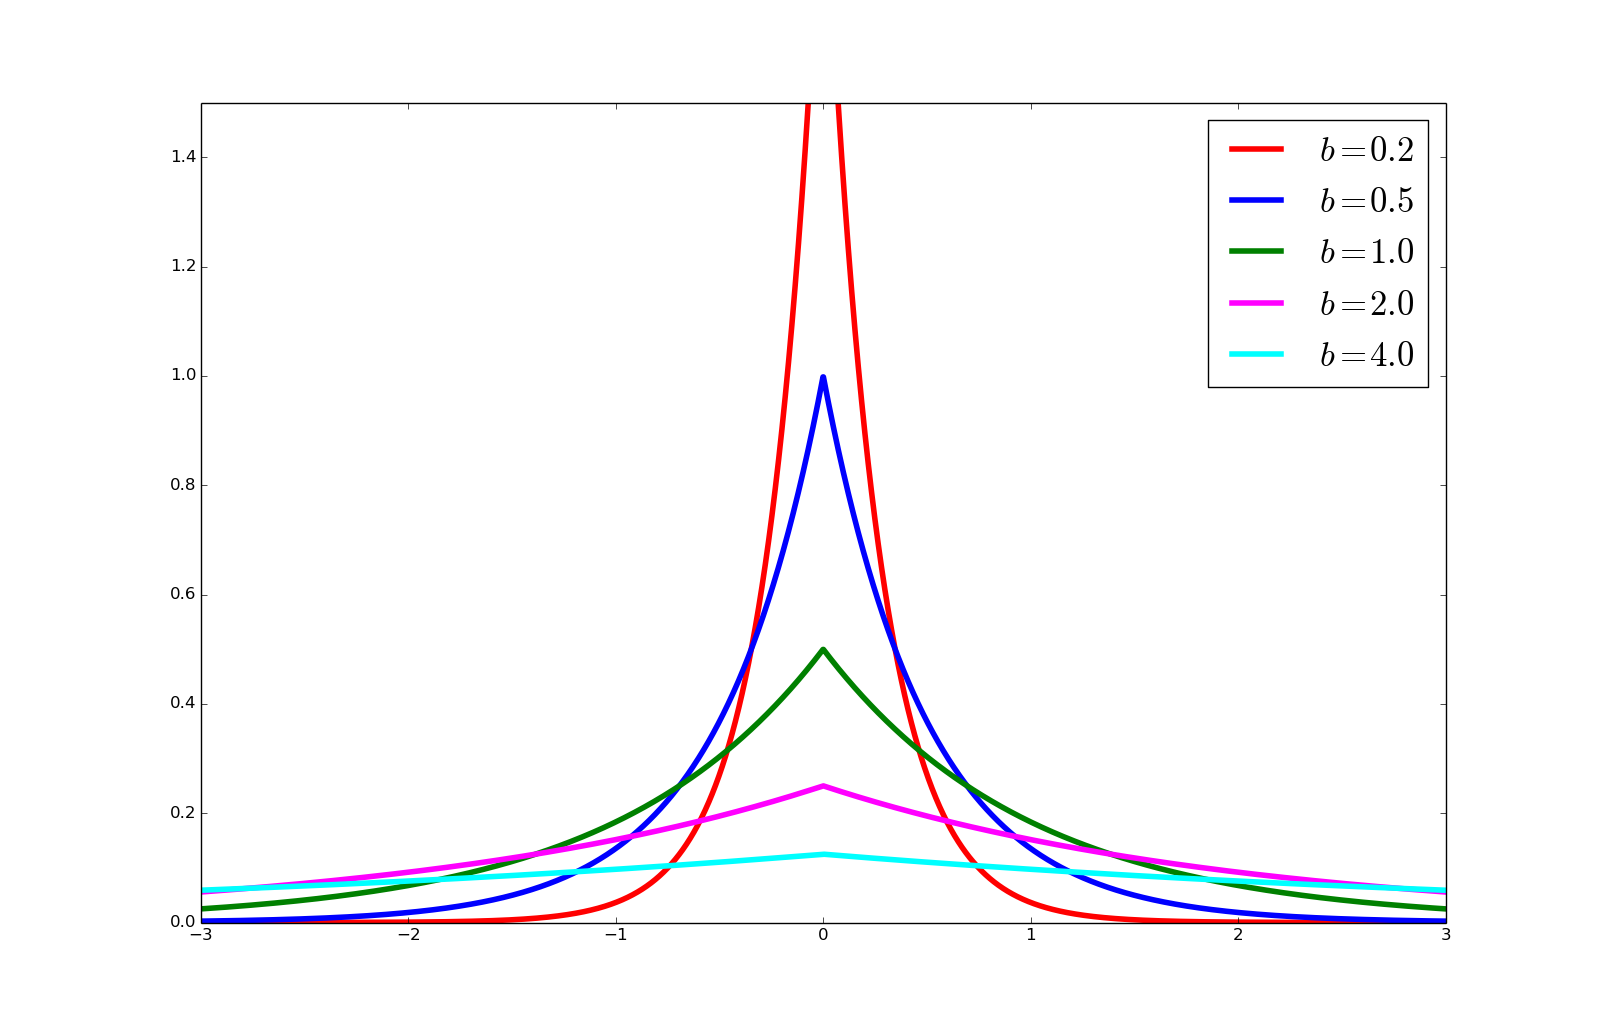
\includegraphics[width=0.75\linewidth]{assets/laplace_b.png}
    \caption{The Laplace distribution centered on zero with different diversity parameters}
    \label{fig:fn_sens}
\end{figure}

\begin{lem}
Any $c$-sensitive function, $f : A \rightarrow \mathbb R$, can be made $\epsilon$-differentially private by adding a value sampled from the Laplace distribution centered on zero with diversity parameter $b=\frac{c}{\epsilon}$.
\end{lem}

Noise sampled from the Laplace distribution scaled according to $b=c/\epsilon$ is sufficient to mask private information while still providing accurate results.

% TODO 1 : rename this section?
\section{PINQ}\label{sec:pinq}

This section provides a brief overview of PINQ and its key components.
PINQ provides differentially-private primitives and operators for composing them into arbitrarily complex, but still differentially private algorithms.
It is layered on top of LINQ, a query EDSL for the .NET family of languages.
There are two main components to PINQ: transformations and aggregations.
Each PINQ server is responsible for maintaining its own privacy budget and rejecting queries whose costs exceed what remains of it.
After a data source's budget has been consumed entirely, it is impossible to query it again through the PINQ interface.

\subsection{Transformations}

LINQ allows users to manipulate data with relational algebra operators directly in the host language.
In LINQ/PINQ terminology, these operations are called transformations.
Our work includes a fully-typed LINQ-like EDSL for Idris which we call RADT. (see \texttt{Database.RADT.Idris}).

PINQ adds a privacy layer around the LINQ query language.
It verifies that query costs do not exceed data source budgets before handing queries off to LINQ for processing.
Many of LINQ's transformations have been made available in PINQ, but some cannot be made differentially private and have been modified or removed.
The word ``stability'' is commonly used when discussing function sensitivity in the context of database transformations.

\begin{cor}[Transformation stability]
A transformation $T$ is $c$-stable if, for all possible pairs of input databases,
$$
  \forall D_1,D_2\in\mathbb D\ldotp |T(D_1)\ominus T(D_2)| \le c \times | D_1 \ominus D_2 |
$$
\end{cor}

See Corrolary~\ref{cor:filterp_1sens} for a proof that $filter_p : \mathbb D \rightarrow \mathbb D$ is 1-stable (sensitive).
Similar proofs exist for all of the other transformations provided by PINQ\cite{conf/sigmod/McSherry09}.
Not all transformations from the LINQ API are $c$-stable for finite values of $c$, preventing them from being usable in differentially private computations.
They have been removed in the PINQ API.
When possible, PINQ provides modified, boundable versions with altered, but still useful semantics.

\subsection{Aggregations}

The only safe way to return information from a sensitive database is to require that it be the result of an aggregation.
PINQ ensures that the only information being released to analysts comes from its carefully implemented aggregation mechanisms.
After evaluating a query with the underlying LINQ provider, every PINQ aggregation will take care to add random noise scaled according a user provided argument: $\epsilon$.

Every aggregation provided by PINQ (and DPDT) is proven to be $\epsilon$-differentially private.
$\epsilon$ allows analysts to fine-tune how they wish to use their allotted privacy budget.
The larger $\epsilon$ is, the more accurate the result will be because the width of the noise distribution scales inversely with $\epsilon$.
However, the cost of evaluating the aggregation scales directly with $\epsilon$ and must be subtracted from the remaining privacy budget.
The total cost of evaluating an aggregation is the product of $\epsilon$ and the stability of the query we run it against.

The simplest of PINQ's aggregation mechanisms is \texttt{noisyCount}, which simply returns the number of rows contained within the given query plus random noise.
A differentially private aggregation is just another function, but it consists of two distinct components: 1) the ``true'' aggregation function and 2) the random noise to be added.
The sensitivity is then the product of the ``true'' sensitivity and $\epsilon$.
The true counting function is 1-sensitive.

\begin{cor}[$trueCount$ sensitivity]
trueCount is a 1-sensitive function.
\end{cor}
\begin{proof}
Consider two databases differing by exactly one row ($D_1 \sim D_2$).
We know the databases differ by only one row, so the distance between the inputs is by definition 1; i.e.

$$d_{in} = d_{\mathbb D}(D_1,D_2)=1$$

The true counts must also then also differ by one; i.e.

$$d_{out} = d_{\mathbb R}(trueCount(D_1),trueCount(D_2))=1$$

Because $d_{in} = d_{out}$, we fix $c=1$ and conclude that \texttt{trueCount} is a 1-sensitive function.
\end{proof}

\begin{cor}
$trueCount$ can be made $\epsilon$-differentially private by adding noise sampled from a Laplacian distribution with $\mu = 0$ and diversity parameter $b=1/\epsilon$.
\end{cor}

Another aggregation mechanism PINQ provides is \texttt{noisyAverage}.
This aggregation poses a unique challenge with respect to function sensitivity.
Assume the existence of an expression function, $r : \texttt{Row} \rightarrow \mathbb R$.
$r$ yields a numeric value for each row and we want the average value resulting from all of the rows contained in the query.
Let $f : \mathbb D \rightarrow \mathbb R$ be the aggregation function which maps $r$ onto all rows and reduces them to their average (i.e. $f = \texttt{average . map r}$).
What is $f$'s sensitivity?

Consider the pair of databases $D_1 \sim D_2$.
They differ by exactly one row.
How much of an effect can that one differing row have on the distance between the output averages?
It is impossible to say with the information we have now.

\begin{cor}[$trueAverage$ sensitivity]
  $trueAverage$ is $\infty$-sensitive.
\end{cor}
\begin{proof}
Imagine a database, $D_1$, containing the ages of bachelors students at a fancy private university, \textit{AB University} (ABU).
In the United States, their ages will most likely range from 18 to 22.
For illustrative purposes, let us assume that $trueAverage(D_1) = 20$.
Alice, who just turned 40 and is tired of how frequently her private data is accidentally made public, has decided to go back to college to study differential privacy.
How will Alice's participation in the database affect $trueAverage(D_2)$, where $D_2$ is $D_1$ plus Alice's records?

It depends on how many students already attend the college.
Let's say it is a small college of just one prior student.
Alice's participation has brought $trueAverage(D_2) = 30$!
College of 20,000?
$trueAverage(D_2) = 20.000999$.
So is $c=10$ or is $c=0.000999$?
And we had to assume that we already knew Alice's age to even get this far!
In reality, we will have no idea what outlier values $r$ might yield.
We are unable to quantify the effect of that one row on the aggregate.
Thus, we must conclude that $trueAverage$ is $\infty$-sensitive.
\end{proof}

PINQ solves this by forcing \texttt{noisyAverage} to clamp values coming from $r$ to the range $[-1,+1]$.
In doing so, PINQ is able to conclude that no row is able to affect the aggregate by more than 2.
It can then be made $\epsilon$-differentially private by adding noise scaled according to $2/\epsilon$.

What if $trueAverage(D) + Lap(2/\epsilon)$ falls outside of $[-1,+1]$?
For very small values of $\epsilon$, the Laplacian distribution is very wide and it is unlikely that the noised result will fall within $[-1,+1]$.
PINQ solves this by generating new noise values over and over again until the constraint is satisfied.
DPDT improves on this behavior by noting that the Laplace cumulative distribution function (CDF), which is used to sample from the Laplace distribution, is invertible.
Where it might typically draw a uniform random variable from the interval $[0,1)$, DPDT instead computes the subinterval for the uniform random variable that guarantees the constraint will be met; e.g. whereas we normally might sample $x \in X=[0,1)$, we can restrict the uniform variable to draw from $X=[0.33,0.75)$ because we know that the noise generated at these bounds will satisfy the original constraint.
See Figure~\ref{fig:lapcdf} for a visualization of constrained sampling.

\begin{figure}
    \centering
    \def\svgwidth{\columnwidth}
    \input{assets/LaplaceCDF.pdf_tex}
    \caption{Visualizing constrained sampling from the Laplace distribution (as in \lstinline{noisyAverage})}
    \label{fig:lapcdf}
\end{figure}

Of course, the decision to clamp values to the interval $[-1,+1]$ will require analysts to pre-process the data before aggregating.
This will require users to explicitly express their assumptions regarding the range of possible values that $r$ could return.
For example, as analysts, if we wanted to compute the average age of the bachelors students at ABU, we might draft a function translating the interval $[18,22]$ (our assumption about their age ranges) to $[-1,+1]$.
Of course, if Alice starts attending ABU as a forty year old, she will be counted in this particular query as a 22 year old.

\chapter{Dependent Types in Idris}\label{sec:dependent_types_in_idris}

Idris is a general purpose, pure functional programming language with dependent types.
Dependent type systems allow types to be predicated on values.
This powerful feature allows developers to assert many aspects of a program in the types which can then be mechanically verified by the compiler.

This section serves as a very brief introduction to dependent types and overview of some of Idris' many interesting language features.
For a more complete introduction, see the Idris tutorial\footnote{http://docs.idris-lang.org/en/latest/tutorial/index.html}.
The reader is assumed to have a basic familiarity with functional programming languages.

We begin with the ``Hello World'' example of dependent types: upgrading the regular \texttt{List a} type to \texttt{Vect n a}.
They share the exact same data representation, but their types are very different.
We then give a brief overview of some Idris language features we make use of in our implementation of DPDT.

\section{Example: Hello Vect}

Just as every introduction to programming tutorial begins with printing ``Hello World'' to the console, introductory dependent types tutorials begin with \texttt{Vect}.
Consider the definition of \texttt{List} in Listing~\ref{lst:lstdef}.
It is \textit{parameterized} by the type of the contained elements (e.g. \texttt{List Double}).
Now consider the (incomplete) definition of \texttt{head}.
It is impossible to satisfy the right-hand side of the first pattern.

\begin{lstlisting}[float,caption={List Definition},label={lst:listdef}]
data List : (elt : Type) -> Type where
  Nil  : List a
  (::) : a -> List a -> List a

head : List a -> a
head []        = ?head_rhs_empty
head (x :: xs) = x
\end{lstlisting}

If a developer were to evaluate the expression \texttt{head []}, it would immediately trigger a runtime exception.
Dependent types allow developers to express assumptions or expectations about functions.
Listing~\ref{lst:vectdef} demonstrates the same \texttt{head} function, but using \texttt{Vect}s instead.
Notice how the definition of \texttt{Vect} is \textit{indexed} by its length and how the type signature of \texttt{(::)} builds the length index constructively with the \texttt{S} data constructor from \texttt{Nat}.
The type signature of \texttt{head} is able to pattern match on that index.
\texttt{Vect (S n) a} can be loosely interpreted as a list of \textit{at least} one element of type \texttt{a}.
\texttt{Vect n a} and \texttt{Vect m a} are not just lists of different lengths, \textit{they are completely different types}.

\begin{lstlisting}[float,caption={Vect Definition},label={lst:vectdef}]
data Nat : Type where
  Z : Nat
  S : Nat -> Nat

data Vect : (len : Nat) -> ( elt : Type) -> Type where
  Nil  : Vect Z a
  (::) : a -> Vect k a -> Vect (S k) a

head : Vect (S n) a -> a
head (x :: xs) = x
\end{lstlisting}

Types are first-class values in Idris.
This means that we can directly manipulate types with as any other term.
Functions can take types as arguments and return types as values.
In fact, dependent type signatures allow for very complex behavior, such as allowing functions to have branching return types (e.g. \texttt{foo : if cond then a else b} is a function returning a value of type \texttt{a} when \texttt{cond} is true.)
Consider the type signatures of \texttt{appendL} and \texttt{appendV} in Listing~\ref{lst:vector_ops_example} to see how useful this can be.
Not only is the type signature of \texttt{appendV} much more descriptive, but Idris is able to verify at compile time that whatever value is returned \textit{must} have length $n + m$.
This can be enormously helpful for reducing developer errors.
Proper use of dependent types can reduce or even eliminate the need for unit testing.

\begin{lstlisting}[float,caption={Vector Operations Example},label={lst:vector_ops_example}]
appendL : List a -> List a -> List a
appendV : Vect n a -> Vect m a -> Vect (n + m) a
\end{lstlisting}

\section{Monadic sequencing and do-notation}

A monad is an abstract structure that represents some sort of computation.
Monads must support two operations: lifting pure elements ``into'' the computation and sequencing two monadic computations.
Each of these operations is implemented differently by each concrete monad instance, but their type signatures alone allow for powerful abstraction.

The \texttt{State} monad is an instance of a monad.
Pure functional languages don't support mutable state, but it can be represented functionally by threading it through a sequence of function calls.
See Listing~\ref{lst:state_example} for an example of threading state with pure functions.

\begin{lstlisting}[float,caption={Threading state through function calls, no monad},label={lst:state_example}]
||| State holding one integer
data MyState = MkState Int

||| Add an int to the state's int
addToState : Int -> MyState -> MyState
addToState x (MkState st) = MkState (x + st)

namespace Examples

  add15 : MyState -> MyState
  add15 = addToState 5 . addToState 10

  foo : Int
  foo = let MkState i = add15 (MkState 0) in i
  -- foo == 15
\end{lstlisting}

The burden of handling the state is left to the developer.
Monads allow us to abstract unnecessary details like that away, allowing developers to focus on \textit{what} the computations are doing rather than how.
Another benefit is that Idris provides monad instances with an alternative syntax for writing monadic code called \texttt{do}-notation.
Idris will simply desugar \texttt{do}-notation syntax to regular function calls.

\begin{lstlisting}[float,caption={Threading state through function calls with do-notation},label={lst:threading_state_do_notation}]
get       : State s s
put       : s -> State s ()
modify    : (s -> s) -> State s ()
evalState : State s a -> s -> a

addToState : Int -> State MyState ()
addToState x = modify (\MkState i => MkState (i + x))

namespace Examples

  add15 : State MyState ()
  add15 = do
    addToState 5
    addToState 10

  foo : Int
  foo = evalState add15 (MkState 0)
  -- foo == 15
\end{lstlisting}

The \texttt{do}-notation allows us to get the state out of the monad context and update it locally before passing it on to the next computation in the sequence.
Idris even allows \texttt{do}-notation for any types overloading the \texttt{return} and $(>>=)$ functions, even if they aren't instances of the \texttt{Monad} typeclass.

In fact, our implementation makes use of this feature.
Monadic sequencing does not allow for the monadic type to change, but we are indexing our computations with their costs.
Every time a private computation is sequenced, the costs must be updated.
But that requires returning a new type, which prevents us from aligning with the monad class.

\section{Implicit arguments and automatic proof search}

Even though Idris' type checker is rather powerful, there are still correct programs that can not be validated by the type checker alone.
The \texttt{List} \lstinline{head} function from earlier is a great example.
The Idris type-checker will not allow us to implement \texttt{head} for \texttt{List}s until we provide it with a proof that the list is not empty.
The type signature of \texttt{head} in Listing~\ref{lst:head_example} shows two arguments: the first is the list and the second is a proof that the list has a head element to return.

\begin{lstlisting}[float,caption={Taking the head of a list},label={lst:head_example}]
head : (xs : List a) -> (isCons xs = True) -> a
head (x :: xs) Refl = x

head : (xs : List a) -> { auto p : isCons xs = True } -> a
head (x :: xs) = x
\end{lstlisting}

For proofs which are easily machine-checkable, Idris allows us to mark them as implicit arguments.
The compiler will automatically search for and provide the correct proof if possible.
In the event that it isn't able to find a sufficient proof, the compiler will abort compilation with a descriptive error message.

Implicit arguments are declared using curly braces.
Adding the \texttt{auto} keyword tells Idris to do a proof search for the required term.
It is possible to specify proof search tactics, but that is rarely necessary.

\chapter{Function Sensitivity in Idris}\label{sec:function_sensitivity}

This chapter demonstrates how we use dependent types to model function sensitivity in Idris.

Recall from Theorem~\ref{thm:csens} that function sensitivity describes how much a function can amplify the distances between pairs of objects.

$$ \forall x,y.\; d(f(x),f(y)) \le c \times d(x,y) $$

\section{Sensitive Function Definition}

We want the type of a sensitive function to describe its sensitivity similarly to how the type of \texttt{Vect} describes its length.
To keep the examples in this chapter simple, we will use \texttt{Float} to represent sensitivity, but DPDT actually uses an abstract representation of \texttt{Rational}s.

Listing~\ref{lst:rep_sens_fns} defines a type constructor indexed by the sensitivity and parameterized by its input and output types.
It has just one data constructor which is used for wrapping native Idris functions.
A \texttt{SensitiveFunction s a b} is a function with sensitivity \texttt{s} mapping tokens from \texttt{a} to \texttt{b}.

\begin{lstlisting}[float,caption={Representing sensitive functions},label={lst:rep_sens_fns}]
||| Represents a sensitive function
||| @ c The sensitivity of the function
||| @ a The input type of the function
||| @ b The output type of the function
data SensitiveFunction : (c:Float) -> (a:Type) -> (b:Type) -> Type where
    MkSensitiveFunction : (a -> b) -> SensitiveFunction s a b

namespace Examples

    add10 : SensitiveFunction 1 Float Float
    add10 = MkSensitiveFunction (+10)

    doubleThenAdd10 : SensitiveFunction 2 Float Float
    doubleThenAdd10 = MkSensitiveFunction (*2)

    cheat : SensitiveFunction 1 Float Float
    cheat = MkSensitiveFunction (*20)
\end{lstlisting}

Notice the \texttt{cheat} example above.
It is possible to define sensitive functions which intentionally misrepresent their sensitivities.
Our focus here is not on the verification of a function's sensitivity, but rather on the interaction between sensitivity and the type system under operations such as function composition and application.

\section{Function Composition and Application}

Unrestricted application is as simple as unwrapping the function and applying it to an argument.
Function composition returns a new type indexed by the combined sensitivities of the underlying functions.
This is done simply by wrapping the composed functions in a new data constructor and computing a new sensitivity index.
Listing~\ref{lst:sens_fns_ops} shows sensitive function composition and unrestricted application.

\begin{lstlisting}[float,caption={Sensitive function operations},label={lst:sens_fns_ops}]
||| Applies a sensitive function to an input
||| @ f The sensitive function to be applied
||| @ x The input
apply : (f:SensitiveFunction s a b) -> (x:a) -> b
apply (MkSensitiveFunction f) x = f x

||| Composes two sensitive functions
||| @ g The outer function
||| @ f The inner function
(.) : (g:SensitiveFunction s b c) -> (f:SensitiveFunction s' a b) -> SensitiveFunction (s*s') a c
(.) (MkSensitiveFunction g) (MkSensitiveFunction f) = MkSensitiveFunction (g . f)
\end{lstlisting}

Now Idris' type-checker understands how sensitive functions compose and it can verify assertions about it.
See Listing~\ref{lst:composition_examples} for examples of how the type-checker verifies sensitivities.

\begin{lstlisting}[float,caption={Examples of Sensitive Function Composition},label={lst:composition_examples}]
doSomeMath : SensitiveFunction 2 Float Float
doSomeMath = add10 . doubleThenAdd10

--doesNotCompile : SensitiveFunction 4 Float Float
--doesNotCompile = add10 . doubleThenAdd10

doSomeMath2 : SensitiveFunction ?sens Float Float
doSomeMath2 = add10 . doubleThenAdd10

Main.sens = proof { intros; search }
\end{lstlisting}

One unfortunate consequence of having such a powerful type-system is that type inference is not possible.
All top-level names must be associated with a type declaration.
This means that despite the type-system being capable of computing the sensitivities, we must still explicitly provide the type, which includes the sensitivity (as in the \texttt{doSomeMath} signature above).
Fortunately, because the computation is decidable (we spent a lot of time with Idris' totality checker and our \texttt{Data.Rational} implementation), users are able to ask Idris for help through its interactive proof search feature.
Asking Idris to find a proof of the hole \texttt{?sens} yields \texttt{fromInteger 2}.
Alternatively, proof tactics can be provided directly in the code (see Listing~\ref{lst:composition_examples}, Line 10).

Listing~\ref{lst:sens_app} demonstrates an alternative application function for sensitive functions.
This one checks whether a function's sensitivity is below the provided value.
Note that this check occurs \textit{at compile time}.

\begin{lstlisting}[float,caption={Sensitivity-aware function application},label={lst:sens_app}]
||| Applies a sensitive function to an input, if its sensitivity does not exceed z
||| @ z The max sensitivity allowed
||| @ f The sensitive function to be applied
||| @ x The input
applyIfLT : (z:Float) -> (f:SensitiveFunction s a b) -> (x:a) -> { auto p : So (s < z) } -> b
applyIfLT _ f x = f x

namespace Examples

    compiles : Float
    compiles = applyIfLT 2 add10 0

    -- doesNotCompile : Float
    -- doesNotCompile = applyIfLT 2 (doubleThenAdd10 . doubleThenAdd10) 0
\end{lstlisting}

\chapter{RADT - Typing the Relational Algebra}\label{sec:RADT}

In this chapter, we review the relational algebra and show how it can be modeled in a dependently typed language.
We first introduce the relational algebra, after which we describe the implementation of our type-safe relational algebra, \textit{Relational Algebra with Dependent Types} (RADT).
Our approach is based on Chapter 4 from \textit{The Power of Pi}\cite{OurySwierstra08PowerOfPi}, an excellent resource for practical examples of what dependent types are capable of.

\section{The Relational Algebra}

The relational algebra describes semantics for modeling and querying data in relational databases (e.g. MySQL\footnote{https://www.mysql.com/}).
E.F. Codd described relational databases and their associated algebra back in the 1970's\cite{codd70}.
The relational model quickly became popular for its simplicity and good performance.

Tables are the fundamental objects which relations build on.
The rows of a table represent individual entities and the columns contain their \textit{attributes}.
Each of these attributes is associated with a name and data type.
Every row (and therefore table) has a \textit{schema}, which is a list of its column names and types.
For example, Table~\ref{tab:people_table} contains four columns; each has a unique name and associated data type.

\begin{table}[tb]
    \caption{People Table}
    \label{tab:people_table}
    \centering

    \begin{tabular}{|c|c|c|c|}
    \hline

    \hline
    \textbf{Key} & \textbf{Name} & \textbf{Age} & \textbf{FavoriteFood} \\
    \hline
    \textit{Int} & \textit{String} & \textit{Int} & \textit{String} \\
    \hline
    \hline
       1 & Casper & 26 & Rogan Josh Curry \\
       2 & Knut & 26 & Moussaka \\
    \hline

    \end{tabular}
\end{table}

The relational algebra allows us to build structured queries against relational databases.
The primary operators are listed below.
Note that some of the operators may require expressions to be provided (e.g. for filtering a table with a conditional).
Our implementation of RADT contains a primitive example of an expression language.

\begin{itemize}
    \item selection
    \item projection
    \item Cartesian product\footnote{\label{fn:set_ops} These operations function identically to their set counterparts, but impose additional requirements regarding table schemas. In particular, union and difference (and therefore intersection) require that the schemas of the two operands match. The Cartesian product operator requires that the two schemas are disjoint.}
    \item union\footnotemark[\ref{fn:set_ops}]
    \item difference\footnotemark[\ref{fn:set_ops}]
\end{itemize}

Note that the set operations and Cartesian product impose additional requirements in this context.
These extra constraints have precluded many type systems from being able to fully type-check the relational algebra.
Strongly-typed languages, such as Haskell, have devised clever solutions to this problem, but none are as straight-forward as the approach available to a dependent type system.
The ability to capture schemas directly in the types and to manipulate them yields a deceptively simple, but powerful typing framework for relational databases.

\section{Our Implementation}

\begin{figure}[H]
\begin{mdframed}
\begin{minipage}[t]{0.5\textwidth}
  \begin{grammar}
    <E> ::= \phantom
    \alt ($\land$) <Schema> <String>
    \alt (+) E E
    \alt \ldots
    \alt Lit <a>
    \alt Couple E E
    \alt PureFn $(a \rightarrow b)$ E

    <Proj> ::= $(String \rightarrow Maybe\ String)$

    <G> ::= \phantom
    \alt groupBy E Q
  \end{grammar}
\end{minipage} % do NOT add a space between this and the next line.
\begin{minipage}[t]{0.5\textwidth}
  \begin{grammar}
    <Q> ::= \phantom
    \alt <t>
    \alt Union Q Q
    \alt Diff Q Q
    \alt Product Q Q
    \alt Project Proj Q
    \alt Select E Q
    \alt Lookup <k> G
    \\

    <P> ::= \phantom
    \alt partitionBy E Q
  \end{grammar}
\end{minipage}
\end{mdframed}
\caption{Informal RADT grammar (refer to \texttt{Database.RADT} for precise specification)}
\label{gram:radt}
\end{figure}

This section provides a brief overview of our implementation of RADT, an EDSL describing the relational algebra in Idris.
Like PINQ, DPDT is implemented as a privacy layer over top of a less restrictive query language.
In this case, that language is RADT, which is based on Oury and Swierstra's approach\cite{OurySwierstra08PowerOfPi}.

Figure~\ref{gram:radt} contains an informal overview of RADT where <E> is just a toy expression language.
The core of the language consists of <Q>, <G>, and <P> which represent queries in various forms (as tables, groupings, and partitionings, respectively).

\subsection{Abstract Representation}

Our foray into RADT begins with some simple algebraic datatypes (ADTs) for describing various components of the system.
Next, we demonstrate an example of the simple expression language before moving on to query representation.

First, we need to represent table attributes (columns).
An \texttt{Attribute} is just the pairing of a name (\texttt{String}) to a data type.
Following David Christiansen's lead\footnote{https://github.com/david-christiansen/idris-type-providers}, we opt to use \texttt{(:::)} instead of the more traditional \texttt{(,)} for constructing our attributes\cite{ChristiansenTypeProviders}.
We believe this enhances readability of long \texttt{Schema}s, which are just lists of \texttt{Attribute}s.

\begin{lstlisting}[caption={Representing attributes and schemas},label={lst:attrs_and_schemas}]
||| Represents an attribute
data Attribute : Type where
  (:::) : String -> Type -> Attribute

||| Represents a schema
Schema : Type
Schema = List Attribute

namespace Examples

    people : Schema
    people = [ "Key"          ::: Int
             , "Name"         ::: String
             , "Age"          ::: Int
             , "FavoriteFood" ::: String
             ]
\end{lstlisting}

The relational algebra assumes the existence of an expression language, so we implement a primitive one for demonstration.
An expression has access to all of a row's attributes during evaluation and can return a value of any type.
So we index expression types by their \texttt{Schema} and parameterize them by the return type.
Thus, an expression with the type \texttt{Expr s a} can be read as an expression with access to the attributes in schema \texttt{s} returning type \texttt{a}.
Notice that we have not yet defined any underlying representation for the rows, but the type is still incredibly descriptive.
In fact, it is completely representation-agnostic (with the exception of \texttt{PureFn}).

Expressions are built up from other expressions, forming an expression tree.
See Figure~\ref{fig:expr_tree} for an example of a simple singly-typed ($\mathbb Z$) expression tree.

\begin{figure}[h!]
    \centering
    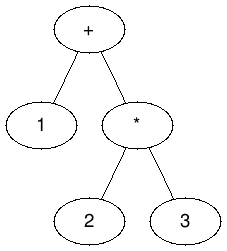
\includegraphics[width=0.25\linewidth]{assets/expr_tree.png}
    \caption{Visualizing expression trees with an example of a simple integer arithmetic expression $(1 + 2 \times 3)$}
    \label{fig:expr_tree}
\end{figure}

% TODO 2 : make a figure of a Query tree showing the types

The return type of the sample tree in Figure~\ref{fig:expr_tree} is obvious, but what about a more complex tree in our expression language?
Expressions cannot change the schema, so that must remain constant even as the tree grows.
The root of the tree represents the final ``operation'' to be evaluated, and therefore the final value.
This value will be returned when the tree is evaluated, so the return type of an expression in RADT is the return type of the root node.
The type-checker is capable of verifying the types throughout the entire tree, so only well-typed expressions are allowed by the type-system.

In fact, the type-checker will even verify that we don't reference attributes that don't exist in a schema (see the dependent type signature: Listing~\ref{lst:expressions}, Line 8).
\texttt{ContainsKey} is a proof that the given schema contains the attribute in question.
It is derived automatically, so users of our language should never have to worry about it.
\texttt{lookupType} is able to use this proof to statically verify the return type of an expression.

\begin{lstlisting}[caption={Abstract representation of toy expression language},label={lst:expressions}]
||| Represents an abstract expression indexed by its schema
||| @ s The schema available to the expression
||| @ a The return type of the expression
data Expr : (s:Schema) -> (a:Type) -> Type where
  ||| Represents a literal value
  Lit    : t -> Expr s t
  ||| Look up a value in the schema
  (^)    : (s:Schema) -> (nm:String) -> { auto p : (map cast s) `ContainsKey` nm } -> Expr s (lookupType s p)
  ||| Represents addition
  (+)    : Num t => Expr s t -> Expr s t -> Expr s t
  ||| Represents equality check
  (==)   : Eq t  => Expr s t -> Expr s t -> Expr s Bool
  ||| Lifts a pure Idris function into the expression language
  PureFn : (a -> b) -> Expr s a -> Expr s b

namespace Examples

  fountain_of_youth : Expr people Int
  fountain_of_youth = people^"Age" - 10

  -- doesNotCompile : Expr people Int
  -- doesNotCompile = people^"Does Not Exist"
\end{lstlisting}

One of PINQ's powerful features is that analysts have access to nearly all of C\#'s capabilities.
We use the \texttt{PureFn} data constructor to lift pure Idris functions into the expression language, allowing users to leverage many of Idris' powerful language features within expressions.
This should allow clever developers to bend even this simple expression language into something quite powerful.
However, this functionality is only available to backends implemented in Idris.

The core of the relational algebra consists of the query operators, which we model as follows.
\texttt{Query} is implemented as a data family, allowing us to adjust its internal data representation just enough to implement a variety of backends.
In particular, the representation of tables is backend specific.
For example, an in-memory Idris backend might store pointers directly to the tables in memory, whereas a SQL backend might just store the name of the table as a string.
Any data source which can be modeled using the relational algebra should be implementable as an RADT backend.

\begin{lstlisting}[caption={Abstract representation of queries},label={lst:queries}]
mutual -- required for mutual definitions

  ||| Represents an abstract query
  ||| @ t A function yielding a base table representation given a schema
  ||| @ s The schema of the query
  data Query : (t:Schema -> Type) -> (s:Schema) -> Type where
    Table   :       t s -> Query t s
    Union   : Query t s -> Query t s -> Query t s
    Diff    : Query t s -> Query t s -> Query t s
    Product : Query t s -> Query t s' -> { auto p : Disjoint s s' } -> Query t (s ++ s')
    Projection : (f:String -> Maybe String) -> Query t s -> Query t (projectedSchema f s)
    Select  : Expr s Bool -> Query t s -> Query t s

  ||| Represents an abstract grouping
  ||| @ t A function yielding a base table representation given a schema
  ||| @ s The schema of the query
  ||| @ k The type of the grouping key
  data Grouping : (t:Schema -> Type) -> (s:Schema) -> (k:Type) -> Type where
    GroupBy : Eq k => Expr s k -> Query t s -> Grouping t s k

  ||| Represents an abstract partitioning
  ||| @ t A function yielding a base table representation given a schema
  ||| @ s The schema of the query
  ||| @ k The type of the partitioning key
  data Partitioning : (t:Schema -> Type) -> (s:Schema) -> (k:Type) -> Type where
    Partition : Eq k => List k -> Expr s k -> Query t s -> Partitioning t s k

namespace Examples

  -- Tables in our Idris backend are: List (Row s)
  ListRow : Schema -> Type
  ListRow s = List (Row s) -- Row defined elsewhere

  -- Tables in our SQLite backend are represented by their names
  SQLiteBackend : Schema -> Type
  SQLiteBackend _ = String
\end{lstlisting}

Recall that the set operators impose additional constraints which have challenged traditional type systems.
Set union and difference require that the two operands share matching schemas and cartesian product requires that they be disjoint.
Type unification allows us to specify the matching schemas constraints very succinctly.
The disjoint proof is slightly more complex; but because it is decidable, it can be automatically derived.

\subsection{Backend Implementations}

We provide two prototype backends with our implementation of RADT: an in-memory Idris-powered backend and a backend compiling SQL query strings targeting SQLite.
However, it is possible to write a backend for any data source which can be modeled with the relational algebra.
One powerful consequence of this is that our privacy layer (DPQ or DPDT) will also work for any relational data source.

There is one caveat: \texttt{PureFn} is only available to Idris-based backends (e.g. an Idris-based server a la LINQ providers).
However, most uses of \texttt{PureFn} could be replaced by extensions to the expression language.
As our abstract representation exists right now, though, it is possible to include \texttt{PureFn}s in an expression intended for a non-Idris backend.
This was an oversight on our part which we aim to fix in the near future.
Until then, backend implementors will need to take care when implementing expression evaluation.

There are two main components required for a functional backend implementation:
1) an underlying table data representation (e.g. ListRow in Listing~\ref{lst:queries}) and
2) evaluator functions for the abstract expression and query trees.
Existing database systems such as \texttt{MySQL}\footnote{https://www.mysql.com/} and \texttt{SQLite} already have their underlying data representations.
Implementing backends for them would likely require compiling abstract syntax trees down to SQL strings which could then be submitted to the database.

Our Idris backend uses a basic \texttt{cons}-list structure indexed over \texttt{Schema}s.
Listing~\ref{lst:idris_backend} demonstrates how we represent databases in-memory (underlying data representation) in Idris.
It also shows snippets from the evaluator functions for both backends.

\begin{lstlisting}[caption={Implementing backends (snippets)},label={lst:idris_backend}]
||| Represents a row of data in memory
||| @ s The row's schema
data Row : (s:Schema) -> Type where
  Nil  : Row []
  (::) : Eq t => t -> Row s -> Row (name:::t::s)

namespace IdrisBackend
  ||| Evaluates an abstract expression in the Idris backend
  evalE : Expr s t -> Row s -> t
  evalE (x + y) r = eval x r + eval y r
    [..]

  ||| Evaluates an abstract query in the Idris backend
  evalQ : (q:Query Table s) -> Table s
  evalQ (Product x y) = [ x' ++ y' | x' <- eval x, y' <- eval y ]
    [..]

namespace SQLiteBackend
  ||| Compiles an abstract expression to a SQLite string
  evalE : Expr s t -> String
  evalE (x + y) = "(" ++ eval x ++ ") + ("  ++ eval y ++ ")"
    [..]

  ||| Compiles an abstract query to a SQLite string
  evalQ : Query SQLiteTable s -> String
  evalQ (Product x y)    = "(" ++ eval x ++ ") , (" ++ eval y ++ ")"
    [..]
\end{lstlisting}

\chapter{DPQ - Differentially Private Queries}\label{sec:DPQ}

\begin{figure}[H]
\begin{mdframed}
\begin{minipage}[t]{0.5\textwidth}
  \begin{grammar}
    <E> ::= \phantom
    \alt ($\land$) <Schema> <String>
    \alt (+) E E
    \alt \ldots
    \alt Lit <a>
    \alt Couple E E
    \alt PureFn $(a \rightarrow b)$ E

    <Proj> ::= $(String \rightarrow Maybe\ String)$

    <G> ::= \phantom
    \alt groupBy E Q

    <A> ::= \phantom
    \alt noisyCount Q $\epsilon$
    \alt noisyAverage Q $\epsilon$
  \end{grammar}
\end{minipage} % do NOT add a space between this and the next line.
\begin{minipage}[t]{0.5\textwidth}
  \begin{grammar}
    <Q> ::= \phantom
    \alt <t>
    \alt Union Q Q
    \alt Diff Q Q
    \alt Product Q Q
    \alt Project Proj Q
    \alt Select E Q
    \alt Lookup <k> G
    \\

    <P> ::= \phantom
    \alt partitionBy E Q
  \end{grammar}
\end{minipage}
\end{mdframed}
\caption{Informal DPQ grammar (refer to \texttt{Database.DPDT} for precise specification)}
\label{gram:radt}
\end{figure}

This chapter describes \textit{Differentially Private Queries} (DPQ), a restricted subset of the DPDT language.
DPQ is just a simple privacy layer wrapped around our implementation of RADT, as described in Chapter~\ref{sec:RADT}.
Sequencing is the primary primitive distinguishing DPQ from DPDT.
Because of this, DPQ is only capable of verifying differential privacy for single queries.
Chapter~\ref{sec:DPDT} builds on this chapter to arrive at our final prototype: DPDT.

Our goal is to leverage the Idris type-checker to statically verify differential privacy constraints in single queries.
We begin by embedding differential privacy metrics into the types as described in Chapter~\ref{sec:function_sensitivity}.
Next, we demonstrate how these sensitivity-indexed types interact with transformations and aggregations.
Finally, we briefly describe the requirements for implementing DPQ-capable backends.

\section{Sensitive Types}

First, we want to wrap our RADT types with new types indexed by their sensitivities.
Listing~\ref{lst:pinqueries} shows how this can be done.
The new types read almost exactly as before, except they are indexed by \texttt{Stability} (type synonym for \texttt{Rational}).

Idris allows name overloading in cases where the correct function can be uniquely identified by the types.
Thanks to this, we don't have to rename our new, sensitive types.
However, to help with reader comprehension, these type names can be prefixed with their respective language when it might be ambiguous (e.g. \texttt{RADT.Query}, \texttt{DPDT.Query}).

\begin{lstlisting}[float,caption={Representing privacy-aware queries},label={lst:pinqueries}]
||| Represents an abstract, stability-aware query
||| @ t A function yielding a base table representation given a schema
||| @ s The schema of the query
||| @ c The stability of the query
data Query : (t:Schema -> Type) -> (s:Schema) -> (c:Stability) -> Type where
    MkQuery : Query t s -> Query t s c

||| Represents an abstract, stability-aware grouping
||| @ t A function yielding a base table representation given a schema
||| @ s The schema of the query
||| @ k The type of the grouping key
||| @ c The stability of the query
data Grouping : (t:Schema -> Type) -> (s:Schema) -> (k:Type) -> (c:Stability) -> Type where
    MkGrouping : Grouping t s k -> Grouping t s k c

||| Represents an abstract, stability-aware partitioning
||| @ t A function yielding a base table representation given a schema
||| @ s The schema of the query
||| @ k The type of the partitioning key
||| @ c The stability of the query
data Partitioning : (t:Schema -> Type) -> (s:Schema) -> (k:Type) -> (c:Stability) -> Type where
    MkPartitioning : Partitioning t s k -> Partitioning t s k c
\end{lstlisting}

We will focus on \texttt{DPDT.Query} because \texttt{DPDT.Grouping} and \texttt{DPDT.Partitioning} have similar implementations, but are case-specific.
A \texttt{DPDT.Query t s c} describes a \texttt{c}-differentially private query with schema \texttt{s} (and backend table representation \texttt{(t s)}).
There is only one data constructor which serves simply to wrap an existing \texttt{RADT.Query}.

\section{Transformations}

Transformations in the DPQ/DPDT privacy layer can change both the schemas and stabilities of queries, but are trivially easy to implement.
First, a transformation must unwrap the underlying \texttt{RADT.Query} objects.
Then, it transforms them using operations from \texttt{RADT}.
Finally, it rewraps the resulting \texttt{RADT.Query} in a \texttt{DPDT.Query} data constructor, \textit{but with a different type constructor}.
This procedure is illustrated in Figure~\ref{fig:query_wrapping}.
At the data level, \texttt{DPDT.Query} isn't terribly interesting; the interesting computations happen at the type level.

\begin{figure}
     \centering
     \def\svgwidth{1\linewidth}
     \input{assets/query_wrapping.pdf_tex}
     \caption{DPQ/DPDT transformation procedure}
     \label{fig:query_wrapping}
\end{figure}

Dependent type signatures allow total computations to be evaluated at compile-time.
We spent significant time fine-tuning totality in the \texttt{Data.Rational} module.
We also spent some time implementing \texttt{projectedSchema} in a manner that is total\footnote{There are some quirks with respect to how Idris reduces terms in dependent signatures. Not all total functions reduce as expected.}.

\begin{lstlisting}[float,caption={Representing privacy-aware transformations},label={lst:transformations}]
||| Represents stability-aware selection
where' : Query b s c -> Expr s Bool -> Query b s c
where' (MkQuery q) e = MkQuery (Select e q)

||| Represents stability-aware projection
select : Query b s c -> (f:String -> Maybe  String) -> Query b (projectedSchema f s) c
select (MkQuery q) f = MkQuery (Projection f q)

||| Represents stability-aware union
union : Query b s c -> Query b s c' -> Query b s (c + c')
union (MkQuery q) (MkQuery q') = MkQuery (Union q q')

||| Represents stability-aware intersection
intersect : Query b s c -> Query b s c' -> Query b s (c + c')
intersect (MkQuery q) (MkQuery q') = MkQuery (Diff q q')

||| Represents stability-aware grouping
groupBy : Eq k => Expr s k -> Query b s c -> Grouping b s k (c * 2)
groupBy e (MkQuery q) = MkGrouping (GroupBy e q)
\end{lstlisting}

Recall from Corollary~\ref{cor:filterp_1sens} that $filter_p$ is 1-sensitive.
In trying to align our implementation with SQL and PINQ naming conventions, $filter_p$ is known as \texttt{where'} in our implementation.
Notice how the type signature of \texttt{where'} reflects that.
The stability index, \texttt{c}, remains unchanged through the rewrapping ($c * 1 = c$).
\texttt{union} is a binary transformation that costs the sum of the costs of its operands.
Notice how this too can be precisely specified in Idris.

\section{Aggregations}\label{seq:DPQ_aggregations}

Of course, we can't just return the results of any query.
A query might just return the database contents untouched, potentially violating every single participant's privacy.
Differential privacy requires that any query response be the result of some sort of aggregation.

DPQ/DPDT does not impose any abstract structure on aggregation operations, as it can be very backend specific.
Both of our backends (Idris, SQLite) implement custom data structures for this detail.
One reason for this is for tracking total computation cost.
Aggregations are $\epsilon$-differentially private, but $\epsilon$ is unbound.
By defining a new type, we can express the notion of a closed computation and index it with the total cost.

Listing \ref{lst:DPQ_aggregations} shows the type declarations for \texttt{Private} in each backend, which represents a private computation indexed by its total cost.
The Idris and SQLite backends implement this structure completely differently.
It also shows a sample aggregation, \texttt{noisyCount}, from each.

\begin{lstlisting}[float,caption={Noisy aggregations}, label={lst:DPQ_aggregations}]
namespace Idris

  data Private : Sensitivity -> Type -> Type
  evalPrivate : Private s a -> PRNG -> a

  noisyCount : (Query ListRow s c) -> (e:Epsilon) -> Private (c*e) Double
  noisyCount (MkQuery q) eps = MkPrivate $ \g =>
    let (rx,g') = rndDouble g
        noise   = samplePure 0 (1 / toFloat eps) rx
        count   = the Double $ fromInteger $ fromNat $ length (eval q)
     in (count + noise, g')

namespace SQLite

  data Private : Sensitivity -> Type
  evalPrivate : Private s -> String

  noisyCount : (Query SQLite s c) -> (e:Epsilon) -> Private (c*e)
  noisyCount  (MkQuery q) eps  =
     let noise = "samplePure(0, " ++ show (1 / toFloat eps) ++ ")"
     in MkPrivate $ "SELECT (COUNT(*) + " ++ noise ++ ") FROM (" ++ eval q ++ ")"
\end{lstlisting}

\section{Backend Requirements}\label{sec:DPQ_requirements}

Any backend implementing DPQ must also meet the requirements for implementing RADT, since we use it for doing the actual transformations.
Additionally, it must provide support for generating Laplacian noise.
This can generally be accomplished via two components: (pseudo)random uniform number generation and the ability to call custom functions.

We implemented a basic C library with the Laplacian distribution and tested it with SQLite (\texttt{util/laplace.c}).
Most common database systems should allow linking with custom C libraries.

\chapter{DPDT - Differentially Private Algorithms}\label{sec:DPDT}

\begin{figure}[H]
\begin{mdframed}
\begin{minipage}[t]{0.5\textwidth}
  \begin{grammar}
    <E> ::= \phantom
    \alt ($\land$) <Schema> <String>
    \alt (+) E E
    \alt \ldots
    \alt Lit <a>
    \alt Couple E E
    \alt PureFn $(a \rightarrow b)$ E

    <Proj> ::= $(String \rightarrow Maybe\ String)$

    <G> ::= \phantom
    \alt groupBy E Q

    <A> ::= \phantom
    \alt noisyCount Q $\epsilon$
    \alt noisyAverage Q $\epsilon$
    \alt $(>>=)$ A A
    \alt return <t>
  \end{grammar}
\end{minipage} % do NOT add a space between this and the next line.
\begin{minipage}[t]{0.5\textwidth}
  \begin{grammar}
    <Q> ::= \phantom
    \alt <t>
    \alt Union Q Q
    \alt Diff Q Q
    \alt Product Q Q
    \alt Project Proj Q
    \alt Select E Q
    \alt Lookup <k> G
    \\

    <P> ::= \phantom
    \alt partitionBy E Q
  \end{grammar}
\end{minipage}
\end{mdframed}
\caption{Informal DPDT grammar (refer to \texttt{Database.DPDT} for precise specification)}
\label{gram:radt}
\end{figure}

DPQ is useful for simple statistical queries that can be represented as one aggregation with the given expression language, but for more complex algorithms this is not sufficient.
We distinguish \textit{queries} from \textit{algorithms} in that they do not support dependent sequencing operations (i.e. conditional branching support).
DPDT implements sequencing for the Idris backend computation type, \texttt{Private}.
Additionally, DPDT supports \texttt{PureFn}, allowing analysts to use many of Idris' own language features alongside DPDT.

\section{Sequencing DPQ}

The structure of \texttt{Private} in DPDT with our Idris backend is just a \textit{State monad}, where the state we are threading through is a random number generator.
The SQLite implementation of \texttt{Private} does not need this as it relies on SQLite's own pseudorandom number generator.

\begin{lstlisting}[float,caption={Representing differentially private mechanisms},label={lst:mechanisms}]
||| Represents a differentially private computation
||| @ c The privacy cost of the computation
||| @ a The return type of the computation
data Private : (c:Sensitivity) -> (a:Type) -> Type
    MkPrivate : (PRNG -> (a,PRNG)) -> Private cost a

||| Lifts a value into a private computation
return : a -> Private 0 a
return x = MkPrivate $ \s => (x,s)

||| Sequences two private computations
(>>=) : Private s a -> (a -> Private s' b) -> Private (s + s') b
(>>=) (MkPrivate sf) f = MkPrivate $ \st => let (x,st1)       = sf st
                                                MkPrivate sf' = f x
                                             in sf' st1

||| Evaluates a private computation
evalPrivate : Private s a -> CrapGen -> a
evalPrivate (MkPrivate f) g = fst (f g)

||| Sequences a Vect of equally expensive private computations
sequence : Vect n (Private s a) -> Private (n * s) (Vect n a)
sequence {s} [] = return []
sequence {n} ps = MkPrivate $ \g =>
  let gs = map snd (unfoldCrapGenN (S n) g)
      vs = (map evalPrivate ps) <*> (init gs)
   in (vs, last gs)

namespace Examples

    nestedAggregations : Private 3 Double
    nestedAggregations = do x <- the (Private 1 Double) someAggregation
                            y <- the (Private 2 Double) someOtherAggr
                            return ((x+y*2)/3)
\end{lstlisting}

Sequencing two queries are additive in cost.
Sequencing computations in functional programming is commonly accomplished using \texttt{Monads}.
In many languages, Idris included, types implementing \texttt{Monad} instances have access to special syntactic sugar, commonly known as \texttt{do}-notation.
\texttt{do}-notation just allows developers to use an alternate syntax for writing monadic code.

We hoped to take advantage of this, but the type signatures required to satisfy a monad instance do not allow the monad type to change.
When we sequence two \texttt{Private} computations, however, we need to produce a new one with a new cost.
Fortunately, Idris does not actually require a \texttt{Monad} instance to overload \texttt{do}-notation.
It just requires that we provide the functions \texttt{$(>>=)$} and \texttt{return}.

Sequencing must index \texttt{Private} correctly, just like the aggregation functions.
Experts are able to write their own aggregations for use with DPDT.
As long as they are using our \texttt{Private} structure, they will be able to freely mix them into sequences of pre-existing DPDT private computations.

In addition to sequencing, DPDT also improves on DPQ by allowing use of the \texttt{PureFn} expression data constructor.
This allows us to use Idris in the expression language, significantly increasing the power of the toy language we outlined in Chapter~\ref{sec:RADT}.

\begin{lstlisting}[float,caption={PureFn expression constructor}, label={lst:purefn}]
PureFn : (a -> b) -> Expr s a -> Expr s b
\end{lstlisting}

One important difference between DPDT and PINQ is the way they track metrics.
Since PINQ is an online, dynamic system, it has at least one trusted runtime server (PINQ provider) tracking a global budget.
When a query is to be evaluated, the privacy layer checks with all data sources whether its cost exceeds their budgets.
PINQ is tracking ``remaining budget''.

Our goal with DPDT is to verify all differential privacy constraints at compile-time.
This very fundamental difference means that DPDT is unable to track ``remaining budget'', because the compiler will only run once\footnote{It may be possible to implement this using type providers.}.
Ultimately, this limits DPDT to tracking ``total computation cost'', where a computation is defined as a single \texttt{Private} object.

It is also important to note that DPDT's differential privacy guarantees apply only within the context of a single \texttt{Private} object.
Each evaluation of \texttt{evalPrivate} is equivalent to resetting the ``budget''.

\chapter{Evaluation}\label{sec:evaluation}

In this chapter, we evaluate our implementation of DPDT.
We begin by introducing some simple queries to gain an intuition for DPQ/DPDT.
Then we verify correct behavior of differentially privacy queries using the DPQ subset of our language (and test RADT by proxy).
Next, we extend our correctness analysis to DPDT by implementing more complex differentially private algorithms.
Finally, we compare DPDT with PINQ and discuss pros and cons of dynamic vs. static verification of differential privacy metrics.

\section{Where in the Database is Alice?}

We begin by manually verifying the behavior of DPDT with simple queries.
There are enough moving parts in a differentially private mechanism to warrant this, but it is also useful for gaining an intuition for DPQ/DPDT.
Listing~\ref{lst:example_data_people} constructs a small database in our Idris backend.

\begin{lstlisting}[float,caption={Building an in-memory database},label={lst:example_data_people}]
import Database.PowerOfPi.Idris

Person : Schema
Person = [ "Name" ::: String , "Age" ::: Double ]

people : Query Person 1
people = mkTable [ [ "Alice"  , 40 ]
                 , [ "Casper" , 26 ]
                 , [ "Knut"   , 26 ]
                 , [ "Tor"    , 26 ]
                 , [ "Gismo"  ,  2 ]
                 ]
\end{lstlisting}

Let us quickly consider some primitive queries and their responses.
First, we will try to determine whether Alice's records are included in the database.
This simple example demonstrates several components of our implementation in action: the expression language, a transformation, and a differentially private mechanism: \texttt{noisyCount}.

\begin{lstlisting}[float,caption={Counting Alices},label={lst:counting_alices}]
countAlices : Private 1 Double
countAlices = do let isAlice = Person^"Name" == Lit "Alice"
                 let alices  = people `where'` isAlice
                 noisyCount alices 1

testCountAlices : IO Double
testCountAlices = evalPrivateIO alices
\end{lstlisting}

\texttt{isAlice} is an \texttt{Expr Person Bool} for finding those rows which contain ``Alice'' in the name column.
\texttt{alices} is a \texttt{PINQuery IdrisTable Person 1}, because \texttt{where'} has a stability of 1.
It abstractly represents the table of participants named ``Alice''.
\texttt{noisyCount} gives us a \texttt{Private} computation.
If we were to modify the cost of it, the Idris type-checker would complain that the cost we specified does not match the true cost.
We could also place a type hole (e.g. \texttt{?howMuch}) and use proof tactics for cost inference.
Finally, when we invoke the \texttt{evalPrivateIO} mechanism, the Idris backend evaluates the query, computes the desired result and adds noise to it before returning it.

Every time we run \texttt{testCountAlices}, we will get a different response because of the Laplacian noise being added to the result.
Given the \texttt{people} table from Listing~\ref{lst:example_data_people}, we can describe from the outset what we expect the distribution of this query to look like (assuming an infinite budget).
Figure~\ref{fig:indistinguishability} shows the PDF curves for \texttt{countAlices} being run on a database with and a database without Alice.
Given a single value sampled from either of those two PDFs, an analyst will have no way of telling which PDF it came from.
We can manually try this by removing Alice from \texttt{people} and rerunning the query.
The results of running \texttt{countAlices} on \texttt{people} and \texttt{tail people} are indistinguishable.

Of course, the analyst could try to sample multiple times and averaging the results to learn the true mean.
DPDT allows this, but the type system ensures that the cost of the query increases accordingly.
Listing~\ref{lst:nested_aggrs} contains an example of how an adversarial analyst might try to bypass our protections.

\begin{lstlisting}[float,caption={Counting Alices (revisited)},label={lst:nested_aggrs}]
alices : PINQuery IdrisTable Person 1
alices = people `where'` (Person^"Name" == Lit "Alice")

tripleCountAlice : Private 3 Double
tripleCountAlice = do x <- noisyCount alices 1
                      y <- noisyCount alices 1
                      z <- noisyCount alices 1
                      return ((x+y+z)/3)

tripleCountAlice' : Private 3 Double
tripleCountAlice' = noisyCount alices 3
\end{lstlisting}

The cost of the computation increases each time the analyst tries to extract information from the database, regardless of how it is used.
In fact, \texttt{tripleCountAlice} and \texttt{tripleCountAlice'} are semantically equivalent.
Averaging the results of three less accurate queries will be just as accurate as the result returned from the same query made three times more expensive.
Put another way, they are asking for the same thing at the same privacy cost; therefore, their representative PDFs will be equal.

Where in the database is Alice?
We don't even know if she is in it.

\section{Verifying Differentially Private Queries}

We verified the correctness of our implementation of DPQ with a variety of techniques.
In particular, we employ unit tests and dependently typed proofs for both backends and some basic integration tests for the SQLite backend.

\subsection{Properties of the Abstract Language}

Types allow us to express assertions about a program using types.
``Program'' in this context does not necessarily mean a whole program source file; it could be just a function or some property of a data type.
This powerful observation is known as the Curry-Howard isomorphism.
The Curry-Howard isomorphism maps propositions to types vice versa.
In order to prove a proposition/type $A$, it is sufficient to produce a value $a : A$.
$a$ is the proof of $A$.

This is a particularly powerful consequence in a dependent type system.
Idris provides many useful types for expressing various propositions about programs.
Consider the return type of \texttt{unionCostsAdd} in Listing~\ref{lst:curryhoward}.
$(=)$ is a type constructor provided by Idris' prelude used for proposing that two terms be equal.
Note that this is not just a dynamic equality check; Idris' type-checker will examine the structures of the types involved and verify the equality.

\texttt{unionCostsAdd} can be viewed as proof that, given two queries with costs $c_1$ and $c_2$, respectively, the union of them will result in a query with cost $c_1 + c_2$.
We never specify what $c_1$ and $c_2$ are, as would be done in unit testing.
Instead, Idris proves the proposition that for all possible pairs of queries, their union \textit{must} result in a query that costs $c_1 + c_2$.

Unit testing proves only that a program is correct for a sampling of the test space.
This is particularly important because we can only write unit tests for cases for which we already have expectations.
There are techniques for identifying corner cases, but they are still only sampling from the test space.

A proof like \texttt{unionCostsAdd} provides a markedly better assurance about the test space because it proves the property across the entire test space.
Our language implementations include various propositions such as these directly in the modules they are defined in.
Their placement there prevents modifications from invalidating properties which should be true.
The type-checker will be unable to verify that the type is inhabited and refuse to compile the module.

\begin{lstlisting}[float,caption={Example of using types to assert properties of programs (Curry-Howard correspondence)},label={lst:curryhoward}]
unionCostsAdd : { q1 : Query b s c1 }
             -> { q2 : Query b s c2 }
             -> { q3 : Query b s c3 }
             -> ( union q1 q2 = q3 )
             -> c1 + c2 = c3
unionCostsAdd Refl = Refl
\end{lstlisting}

In addition to proofs about DPQ/DPDT language constructs, we implemented a number of proofs about \texttt{Rational} properties.
Convincing Idris that operations on \texttt{Rational}s are completely total was difficult, but by expressing our expectations as propositional proofs, we were able to identify the problem spots.
Listing~\ref{lst:reductionprfs} shows how we were able to propose reduction properties about operations.

\begin{lstlisting}[float,caption={Examples of reduction property proofs for \texttt{Rational}s},label={lst:reductionprfs}]
fromDec_reduces : (d:Dec b) -> fromDec Z Z d = Z
fromDec_reduces (Yes _) = Refl
fromDec_reduces (No  _) = Refl

rationalsReduce : (4//8) = 1//2
rationalsReduce = Refl

rationalsReduceWhenAdded : (1//4) + (1//2) = (3//4)
rationalsReduceWhenAdded = Refl
\end{lstlisting}

\subsection{Testing the Idris Backend}

We have a combination of unit tests and proofs for verifying that our Idris backend operates as expected.
Most of the property proofs exist directly in the modules they are most relevent to.
The unit tests live in the /tests/idris/ directory.
Because the Idris backend can so easily be tested, we provide a script which should be used by developers for compiling all of the test files as a git pre-commit hook.

Being able to express expectations so clearly was incredibly useful during our exploration phase in implementing DPDT.
We did not have to spend any time on writing unit tests and the compiler itself complained when we violated our expectations.
Listing~\ref{lst:privprops} contains two properties which were particularly useful for debugging.

\begin{lstlisting}[float,caption={Properties of \texttt{Private} computation sequencing},label={lst:privprops}]
returnIsFree : { p1 : Private s1 Double } -> { p2 : Private s2 Double }
            -> do { x <- p1; return 1.0 } = p2 -> s1 = s2
returnIsFree Refl = Refl

sequencingIsAdditive : { p1 : Private s1 a } -> { p2 : Private s2 a }
                    -> { p3 : Private s3 (a,a)  }
                    -> do { x <- p1; y <- p2; return (x,y) } = p3 -> s1 + s2 = s3
sequencingIsAdditive Refl = Refl
\end{lstlisting}

We also wrote a simple, but complete program that loads real data into the backend database and then runs a differentially private aggregation against it.
Please see Listing~\ref{appx:aoldata_idris} in the appendices.

\subsection{Testing the SQLite Backend}

Similarly to our Idris backend, we provide a number of unit tests for the SQLite backend.
Listing~\ref{lst:example_DPQ_unit_test} contains a snippet from one of our unit test modules.
We verify that total costs are calculated as expected with in the SQLite \texttt{Private} type.
We also verify that a specific query compiles to an expected query string.
Notice how $(=)$ can also be used for implementing unit tests.
Also be aware the \texttt{countThemAll} is not a unit test!
But it is testing that our type system behaves as expected.
If we changed the cost of \texttt{countThemAll}, the Idris type-checker would be unable to unify the incorrect cost with the correct one.

\begin{lstlisting}[float,caption={Unit test for noisyCount},label={lst:example_DPQ_unit_test}]
Person : Schema
Person = [ "Name" ::: String , "Age" ::: Nat ]

people : Query Person 1
people = mkTable "People"

countThemAll : Private 2
countThemAll = noisyCount people 2

countThemAllTest : evalPrivate countThemAll = "SELECT (COUNT(*) + samplePure(0, 0.5)) FROM (People)"
countThemAllTest = Refl
\end{lstlisting}

The expected query string in Listing~\ref{lst:example_DPQ_unit_test} contains an example usage of a function from our external C library, \texttt{samplePure}.
SQLite does not provide the Laplacian distribution in its libraries, so we must manually provide it.

We also created some basic integration tests for testing with a real SQLite database.
We use C++ to load a SQLite database, link it with our C library, and run compiled DPQ queries against it.

Additionally, we have manually tested that, assuming an infinite budget, the mean of repeated noisy aggregations approach the true mean.
This ``sanity check'' allows us to be reasonably certain that the interface between our dependent type safety and the outside world behaves as expected.

% TODO 1 : better title?
\section{DPDT vs. PINQ: The Final Showdown}

\subsection{Purity vs. Side Effects}

One of LINQ's key features is that it is embedded within the .NET languages.
This means that developers have access to much more than the LINQ DSL when writing applications; they are able to use all of the features of the host language.
This is a very powerful feature that allows users to seamlessly blend data access and flow control in one environment.

DPDT exists as an embedded language within Idris.
However, there are important differences between an imperative language like C\# and a pure functional language like Idris.
In particular, C\# makes no effort to contain side effects or limit access to global state.
Idris, on the other hand, offers us \textit{referential transparency}; i.e. an expression can be replaced by its value without affecting the semantics of the program at all.

This may seem unimportant, but side effecting functions can compromise differential privacy in spectacular ways.
Consider the result of the following expression.

\begin{lstlisting}[float,caption={Example side-channel attack}]
patients.Select(p => if p.Name == "Alice" {
                        beep();
                     };
                     return p;
);
\end{lstlisting}

The result is a no-op: the data remains unchanged.
However, if the analyst hears a beep during the evaluation of this query, he knows that Alice is included in the \texttt{patients} database.
In fact, beep is just one example of a side-channel.
Other possible examples include timing attacks (e.g. \texttt{Thread.sleep}), writing to global memory or external file (e.g. \texttt{echo yes > /foundAlice}), or even sending an email.
These kinds of interactions with the outside world are called \textit{side effects}.

PINQ does attempt to examine all expressions before evaluating them for potential side-effects, but this approach is error-prone and mechanically deciding whether an expression could violate privacy constraints is difficult.

Idris' type system does not allow functions to contain side effects unless they are explicitly marked as such in their type signature.
This alone prevents many of the side-channel attacks that are possible in other systems.
The types prevent malicious users from tricking the system into writing Alice's private records to a file.

One side-channel which even Idris is susceptible to is a special class of timing attack.
Idris will prevent an expression developer from making calls to \texttt{Thread.Sleep} and similar functions, but Idris is unable to predetermine the running time of an expression.
Instead of calling \texttt{beep()} in the example above, the analyst could have asked for the prime factorization of some very large number.
If he observes that a query takes significantly longer than it did without the call to the expensive computation, he can conclude that Alice's records are in the database.
Stopping this kind of side-channel attack requires a dedicated runtime system which ensures that, regardless of which row the expression is evaluated on, it takes the same amount of time\cite{conf/uss/HaeberlenPN11}.

\subsection{Static vs. Dynamic Differential Privacy}

Alone, DPDT leverages Idris' powerful type system to statically verify the differential privacy constraints of a query.
Combining DPDT with Idris, however, gives it access to all of the features of a Turing complete language.
It is no longer restricted to simple queries.
We can write differentially private algorithms a la PINQ and prevent some of the side channel attacks it might have been susceptible to.

However, using dependent types to verify differential privacy metrics does prevent some types of algorithms from being expressible in DPDT.
This is because we must know the total cost in order to fully construct a computation's type.
If the type-checker is unable to determine when an algorithm will terminate statically, it is impossible to assign it a type.
Our implementation of k-means runs for a fixed number of iterations.
Computing the total cost of running it is accomplished by multiplying the cost of an iteration with the total number of iterations.

However, k-means can also be implemented to use a criteria function for dynamic termination.
It is impossible for the type-checker to know when this variation will terminate, or if it even will.
DPDT's type system precludes dynamically terminating algorithms from being expressed.

PINQ is able to represent dynamic k-means by relying on the fact that geometric series with $-1 < r < 1$ converge.
If each iteration uses exactly half of the remaining budget ($r=1/2$), then the cost of the entire algorithm, regardless of how many iterations are necessary, cannot exceed the budget.

$$\sum_{x=2}^{\infty} 1/x = \frac{1}{2} + \frac{1}{4} + \frac{1}{8} + .. = 1$$

It may be possible for us to extend the \texttt{Sensitivity} type and convince the Idris type-checker that algorithms resembling a geometric series with $-1 < r < 1$ converge, but we have not yet explored this option.

\chapter{Conclusion}\label{sec:conclusion}

Nicolas Oury and Wouter Swierstra demonstrated that dependent types are a natural fit for fully typing the relational algebra\cite{OurySwierstra08PowerOfPi}.
Chapter~\ref{sec:RADT} provided an overview of our implementation of RADT, which was based on their work.

The primary goal of this thesis has been to demonstrate that dependent types also can be used for typing differential privacy metrics and we certainly believe this to be the case.
Chapter~\ref{sec:function_sensitivity} showed how easily metrics such as function sensitivity can be tracked using dependent types.
Chapter~\ref{sec:DPQ} outlined our implementation of a subset of DPDT's features, which we refer to as DPQ.
DPQ is a fully-type safe query DSL for describing one differentially private aggregation at a time.
This subset of features is enough to allow compilation to SQL strings for use in other applications.
In Chapter~\ref{sec:DPDT}, we add sequencing and, for the Idris backend, the ability to lift Idris functions into the expression language, resulting in a PINQ-like language: DPDT.
DPDT is a prototype EDSL for describing differentially private queries in Idris.

\section{Type Safety}

LINQ provides type-safety for most of the relational algebra.
PINQ expands this safety to include privacy metrics, but it does so dynamically.
This actually allows PINQ to express some forms of algorithms which aren't possible in DPDT.
Any algorithm relying on dynamic conditions for termination will be difficult to statically verify.
How can the type-checker know the cost of an algorithm when it could run for any number of iterations?

DPDT provides type-safety for all of the relational algebra and differential privacy constraints.
Two powerful consequences of this are that type-correct programs written in DPDT are guaranteed to be differentially private and will terminate with a result (not a runtime budget error).

In fact, DPDT's type-safety even protects against many side-channel attacks which might be possible in a side-effecting language like PINQ.
PINQ does try to ``scrub'' any expressions before they are evaluated, but mechanically determining which expressions constitute a side-channel attack is not feasible.
However, timing attacks represent one side-channel which no type system is likely to be able to stop.
Certainly, Idris' purity will prevent calls to \texttt{Thread.sleep}, but what about an expression computing the $n^{th}$ Fibonacci number for some large $n$?
A specialized runtime system is required to prevent this kind of side-channel attack\cite{conf/uss/HaeberlenPN11}.

Dependent type systems have benefited from decades of research and come a long way from their academic origins.
Languages like Agda\footnote{http://wiki.portal.chalmers.se/agda/pmwiki.php}, and more recently, Idris, combine the power of dependent types with a powerful, Turing-complete functional programming languages (computations at the type level are not Turing-complete).
This yields a very practical setting for developing differentially private algorithms.

We believe that despite the limitations regarding dynamically-terminating algorithms, dependent types are a great match for representing differential privacy metrics.
We provide DPQ and DPDT as concrete prototype EDSLs demonstrating this, as well as several example programs written with them.

\section{Future Work}\label{sec:future_work}

DPDT is still just a prototype, so there are many potential paths for future work.
We list what we see as the most promising ones here.

\paragraph{Some algorithms can be implemented in PINQ but not DPDT.}
Dynamically terminating algorithms are by definition difficult to analyze statically.
DPDT's current type system precludes all dynamically terminating algorithms.
PINQ is able to implement dynamic kMeans in the case where the iterative costs resemble a geometric series with $-1 < r < 1$.
We believe that it may be possible to extend \texttt{Rational}s in such a way that Idris' type-checker could unify costs appropriately.

\paragraph{Implement new DPDT ``providers'' for other data sources.}
Backends don't need to be limited to local memory access.
A DPDT server component, not unlike many network-facing LINQ providers, would help DPDT better mirror PINQ's capabilities.
By establishing a trusted runtime system on the server hosting the data, we can expose the powers of \texttt{PureFn} to data analysts remotely.

%%%%%%%

\paragraph{Explore Idris language features for other ways to improve DPDT.}
Idris serves as a test bed for several new and interesting experimental language features which could provide DPDT with better integration into its host language.
Two examples that come to mind are Idris' \texttt{Effects} library and \textit{type providers}.

Effects are an alternative to monadic actions for describing side-effects.
Reimplementing the \texttt{Private} monad from Chapter~\ref{sec:DPDT} using effects would be more idiomatic for integration into Idris.
There may be other opportunities for implementing components of randomized mechanisms as effects.

Type providers allow the Idris type-system to define and predicate types based on input from the outside world.
A common use case for type providers is communicating directly with a database for getting schemas.
This could be extended for getting remaining privacy budget.

\paragraph{The expression language is not type-safe because of \texttt{PureFn}}.
DPDT's implementation should be adjusted so that \texttt{PureFn} is disabled for backends which do not support it.
The current implementation will quit with a runtime error.

%%%%%%%

\paragraph{DPDT syntax is far from ideal.}
In its current form, it is not particularly well suited to users who aren't familiar with Idris' syntax or functional programming.
However, Idris tries to make embedding domain specific languages easier by allowing developers to modify its parser and elaborator.
Custom syntax rules allow embedded language developers to extend the parser with EDSL-specific syntax constructs.

Idris syntax extensions consist of two components: reserved keywords and non-terminals.
Keywords help anchor the parser around the non-terminals, which are captured and usable on the right hand side of a custom syntax declaration.
Listing~\ref{lst:syntax_extensions} contains two examples of syntax rules.

\begin{lstlisting}[caption={Extending Idris' syntax},label={lst:syntax_extensions}]
-- Definition
syntax select [f] from [q] = select q f
syntax select [f] from [q] where [e] = select (where q e) f

-- Application
select f from (q `union` q') where e
\end{lstlisting}

In fact, it may be possible to recreate a SQL-like syntax using Idris parser extensions exclusively.
They should, however, be used with caution as poorly implemented syntax rules can cause the parser to diverge.

\section{Closing Remarks}

Dependent types are capable of representing differential privacy metrics and constraints.
The ability to verify differential privacy by construction is a desirable property.
PINQ has demonstrated one method for achieving this, but PINQ relies on dynamic checks for private computations.
DPDT aims to provide the same differential privacy guarantees as PINQ by allowing users to compose complex algorithms from secure primitives, but with improved type-safety.
By lifting the privacy concerns into the type-system, DPDT is able to statically verify a differentially private program at compile-time.
Any program written in DPDT is guaranteed to be differentially private, because the compiler will reject any which aren't.

PINQ can accomodate some types of algorithms which aren't possible in DPDT.
This is an unfortunate consequence of requiring that it statically verify all differential privacy costs at compile time.
We have shown that dependent types are capable of handling differentially private queries (as opposed to algorithms).
Independent queries can be run in any order and may as well be considered a single query costing the sum of the subqueries' costs.
The same is true of a sequence of dependent queries if we know its exact length.
However, DPDT can't know how many iterations a dynamically-terminating algorithm will require, so it won't be able to type that kind of algorithm.
Some improvements to DPDT's understanding of costs might be possible, but some classes of algorithms will not be possible without relaxing the requirements.

Despite these limitations, DPDT's type-system does offer some benefits over that of PINQ's.
In particular, because it is a pure language, almost all side-channel attacks that might be possible in PINQ are prevented by default.
Unfortunately, both PINQ and DPDT are susceptible to a particular form of timing attack: careful use of expensive computations.
Preventing this kind of attack requires a smart server implementation like the one described in \cite{conf/uss/HaeberlenPN11}.

Dependent types can fully represent the relational algebra and its contraints which have stumped lesser type-systems\cite{OurySwierstra08PowerOfPi}.
We have shown that dependent types can also represent differential privacy metrics and their constraints---with some limitations on the types of algorithms that can be expressed.
There are no limits on constructing independent, differentially-private queries, but dynamically terminating algorithms cannot be expressed because privacy constraints cannot be verified at compile-time.
Despite this limitation, we believe that dependent types lend themselves quite well to representing differential privacy metrics and constraints.

\bibliographystyle{abbrv}
\bibliography{main}

\begin{appendices}

\chapter{Sample Programs}

\begin{lstlisting}[caption={tests/Idris/AOLData.idr},label={appx:aoldata_idris}]
module Main

import Database.DPDT.Idris

AOLSchema : Schema
AOLSchema = [ "AnonID" ::: String, "Query" ::: String ]

parseLine : String -> Row AOLSchema
parseLine cs = let (x::y::zs) = split (== ',') cs
                in [ x , y ]

loadTable : String -> IO (Query AOLSchema 1)
loadTable fname = do
  f <- map parseLine . lines <$> readFile fname
  return $ MkQuery (Table f)

-- TODO 1 : FIX THIS! We need associativity: esp. with (fromInteger 1). Commutativity would be nice, too.
-- (Try changing c*2*1 to anything else.)

countUniqueAnonID : Query AOLSchema c -> Private (c*2*1) Double
countUniqueAnonID q = do
  let gq = groupBy (AOLSchema^"AnonID") q
  noisyCount gq 1

main : IO ()
main = do
  t <- loadTable "tests/AOL_sm.txt"
  print $ evalPrivate (countUniqueAnonID t) 1238389612
  return ()

\end{lstlisting}

\begin{lstlisting}[caption={tests/SQLite/AOLData.idr},label={appx:aoldata_sqlite}]
module Main

import Database.DPDT.SQLite
import Effects
import Effect.StdIO

AOLSchema : Schema
AOLSchema = [ "AnonID" ::: Double, "Query" ::: String ]

table : Query AOLSchema 1
table = MkQuery (Table "AOL")

countUniqueAnonId : Private 2
countUniqueAnonId =
  noisyCount gq 1 where
  gq : Grouping AOLSchema Double 2
  gq = groupBy (AOLSchema^"AnonID") table

averageAnonId : Private 1
averageAnonId = noisyAverage (AOLSchema^"AnonID") table 1

printResult : Eff () [STDIO]
printResult = do
              putStr $ evalPrivate countUniqueAnonId ++ "\n"
              putStr $ evalPrivate averageAnonId ++ "\n"

main : IO ()
main = run printResult
\end{lstlisting}

\begin{lstlisting}[caption={tests/idris/kMeans3.idr},label={appx:kMeans3}]
module Main

import Data.Vect
import Database.DPDT.Idris
import Data.Floats
import System.Random.CrapGen

----------------------------------------------------------------

record Point2 where
  constructor MkPt
  ptX : Double
  ptY : Double

dist : Point2 -> Point2 -> Double
dist (MkPt x y) (MkPt x' y') = sqrt $ (x-x')*(x-x') + (y-y')*(y-y')

instance Eq Point2 where
    (==) x y = dist x y < (1/1000000)

----------------------------------------------------------------

SPoint2 : Schema
SPoint2 = [ "x" ::: Double, "y" ::: Double ]

----------------------------------------------------------------

points : Query SPoint2 1
points = MkQuery $ Table $ [ point2 x y | x <- [0,1], y <- [0,1] ]
                        ++ [ point2 x y | x <- [7,8], y <- [7,8] ]
  where point2 : Cast a Double => a -> a -> Row SPoint2
        point2 x y = [ (cast x), (cast y) ]

----------------------------------------------------------------

labelVect : Vect n a -> Vect n (Nat,a)
labelVect v = go v Z
  where go : Vect n a -> Nat -> Vect n (Nat,a)
        go [] k        = []
        go (x :: xs) k = (k,x) :: go xs (S k)

-- classifies each point and gives an ix to the center it matched
classify : Vect (S n) Point2 -> Point2 -> Fin (S n)
classify {n} cs p = let ds = map (dist p) cs
                     in fromNat . fst $ foldr1 findMinDist (labelVect ds)
  where findMinDist : (Nat,Double) -> (Nat,Double) -> (Nat,Double)
        findMinDist (ix,d) (ix',d') = if (d < d') then (ix,d) else (ix',d')

eps : Epsilon
eps = (1//2)

updateCenters : Vect (S n) Point2 -> Grouping SPoint2 (Fin (S n)) c
             -> Private ?updateCenters_cost (Vect (S n) Point2)
updateCenters cs gr = sequence (map (updateCenter gr) (map (fromNat . fst) $ labelVect cs))
  where
    updateCenter : Grouping SPoint2 (Fin (S n)) c -> Fin (S n) -> Private (c*eps + c*eps) Point2
    updateCenter gr ix = do
      let ps = lookup ix gr
      x <- noisyAverage (SPoint2^"x") ps eps
      y <- noisyAverage (SPoint2^"y") ps eps
      return (MkPt x y)

kMeans : (k:Nat) -> (cs:Vect (S n) Point2) -> (tbl:Query SPoint2 1) -> Private ?kMeans_cost (Vect (S n) Point2)
kMeans Z     cs tbl = return cs
kMeans (S k) cs tbl = do
    cs' <- updateCenters cs (groupBy classifyExpr tbl)
    kMeans k cs' tbl
  where classifyExpr = PureFn (classify cs) (PureFn (uncurry MkPt) (Couple (SPoint2^"x") (SPoint2^"y")))

foo : Vect 2 Point2
foo = evalPrivate (kMeans 10 [MkPt 3 4, MkPt 5 6] points) 123

---------- Proofs ----------

Main.updateCenters_cost = proof
  intros
  search

testDist : dist (MkPt 0 0) (MkPt 0 1) = 1
testDist = Refl
\end{lstlisting}

\end{appendices}

\end{document}
